\chapter{Modelando la incertidumbre}
\label{sec:algoritmo}
%\section{Agregando probabilidades a un algoritmo existente}
 Las posibles aplicaciones de la generaci\'on de expresiones referenciales que deben referirse al mundo real sufren de \textbf{incertidumbre} por datos ruidosos de sensores y modelos incompletos de la realidad como discutimos en el Cap\'itulo \ref{sec:intro}.
En este cap\'itulo se presentan nuevos algoritmos basados en teor\'ia de modelos y $\+L$-simulaciones como los descriptos en el Cap\'itulo \ref{sec:intro_logica}. Pero que a diferencia de estos usan una distribuci\'on de finita de probabilidades que representa esta incertidumbre. Estos algoritmos generan no \textbf{una} ER, sino un \textbf{ranking} de ERs. Este ranking de expresiones referenciales est\'a ordenado por la probabilidad de ser correctamente interpretada en el contexto. 
Conseguimos as\'i tres caracter\'isticas nuevas de estos algoritmos:
\begin{itemize}
 \item \textbf{No determinismo}: dos ejecuciones del algoritmo con la
misma entrada podr\'{i}an resultar en diferentes ERs para los objetos en la escena. Podemos generar entonces como salida un ranking de las ERs generadas por el algoritmo si lo ejecutamos muchas veces con
el mismo input. 
 \item Conseguimos mayor control sobre la sobreespecificaci\'on que genera el algoritmo, simulando el tipo y la cantidad de sobreespecificaci\'on que encontramos en  corpora.
 \item Dado un corpus de ERs para un dominio determinado,
es posible usar aprendizaje autom\'atico para aproximar una distribuci\'on de probabilidad adecuada para las propiedades y relaciones de una escena no vista antes. Esto hace que el ranking de las ERs generadas para el modelo simule el que se observa en el corpus.
\end{itemize}

El cap\'itulo est\'a dividido en cinco secciones. En la primer secci\'on explicaremos la entrada y salida del algoritmo. En la Secci\'on \ref{sec:learning} mostraremos como obtener la distribuci\'on de probabilidad finita que toma como entrada el algoritmo, usando aprendizaje autom\'atico cuando hay corpus disponible para la escena. Luego en la Secci\'on \ref{sec:algoritmo_probabilistico} mostraremos el algoritmo en detalle, definiremos los conceptos y t\'ecnicas de teor\'ia de modelos necesarios para entenderlo. En la Secci\'on \ref{sec:ejemplo_ejecucion} mostramos un ejemplo de ejecuci\'on paso a paso. Explicaremos c\'omo conseguimos asegurar terminaci\'on, c\'omo se generan las ERs no-determin\'isticamente y c\'omo conseguimos mayor control sobre la sobreespecificaci\'on. Finalmente en la Secci\'on \ref{sec:link-algoritmo} daremos un res\'umen y comentamos como se linkea el cap\'itulo con el resto de la tesis.

\section{Entrada y salida del algoritmo probabil\'istico}
\label{input_algo}
El sistema toma como entrada un contexto representado por un \textbf{modelo} $\+M$, ---por ejemplo en la Figura \ref{figura-y-modelo} se muestra el modelo de la escena de la izquierda--- el \textbf{target}, recordemos que el target podr\'a ser singular si es un conjunto singleton o plural cuando contenga m\'as de un elemento ---en la figura es el conjunto singleton \{$e_5$\}. 
\begin{figure}[H]
\begin{subfigure}{.5\textwidth}
  \centering
	%\vspace*{-.2cm}
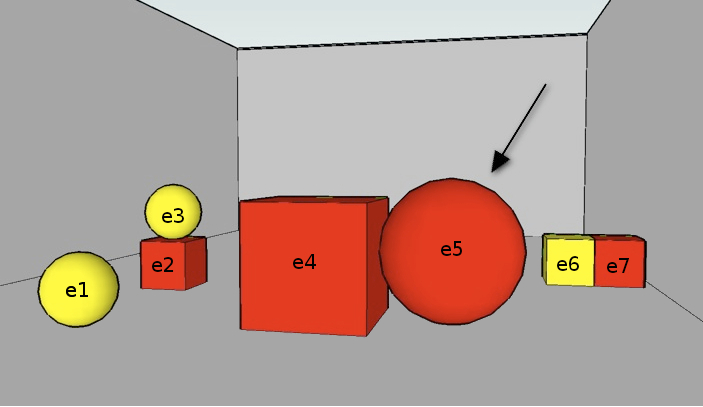
\includegraphics[width=\textwidth]{images/22.jpg}
 % \caption{}\label{GRE3D7-stimulus1-ids-modelo-y-figura}
\end{subfigure}
\begin{subfigure}{.5\textwidth}
  \centering
%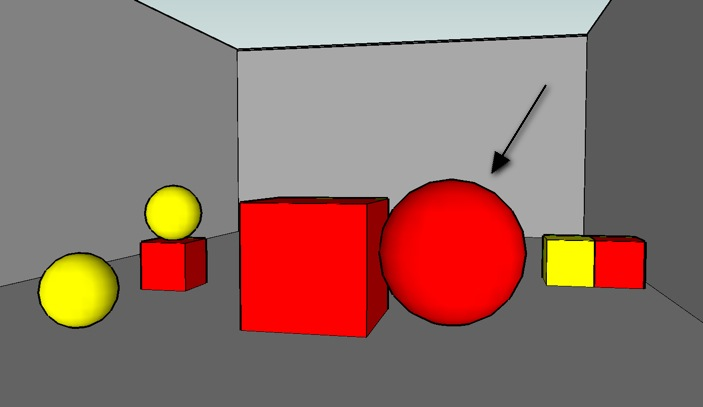
\includegraphics[width=\textwidth]{images/22sinletras.jpg}
%%\caption{Ejemplo de contexto}
%\label{GRE3D7-stimulus1-b}
\vspace*{1cm}
\begin{picture}(250,0)
\put(0,-50){\begin{tikzpicture}
  [
    n/.style={circle,draw,inner sep=1.5pt,node distance=1.5cm},
		 aArrow/.style={->, >=stealth, semithick, shorten <= 1pt, shorten >= 1pt},
  ]
 \node[n,label=below:{
    \relsize{-2}$\begin{array}{c}
      \nSmall\\[-3pt] 
      \nYellow \\[-3pt] 
      \nBall\end{array}$}] (a) {$e_1$};
 \node[n,label=below:{
    \relsize{-2}$\begin{array}{c}     
      \nSmall\\[-3pt] 
      \nRed\\[-3pt] 
      \nCube\end{array}$}, right of=a] (b) {$e_2$};
 \node[n,label=above:{
    \relsize{-2}$\begin{array}{c}     
      \nSmall\\[-3pt] 
      \nYellow\\[-3pt] 
      \nBall\end{array}$}, above of=b] (c) {$e_3$};
 \node[n,label=below:{
    \relsize{-2}$\begin{array}{c}
      \nLarge\\[-3pt] 
      \nRed\\[-3pt] 
      \nCube\end{array}$}, right of=b] (d) {$e_4$};
 \node[n,label=below:{
    \relsize{-2}$\begin{array}{c}
      \nLarge\\[-3pt] 
      \nRed\\[-3pt] 
      \nBall\end{array}$}, right of=d] (e) {$e_5$};
 \node[n,label=below:{
    \relsize{-2}$\begin{array}{c}
      \nSmall\\[-3pt] 
      \nYellow\\[-3pt] 
      \nCube\end{array}$}, right of=e] (f) {$e_6$};
 \node[n,label=below:{
    \relsize{-2}$\begin{array}{c}
      \nSmall\\[-3pt]
      \nRed\\[-3pt] 
      \nCube\end{array}$},  right of=f] (g) {$e_7$};
 \draw [aArrow,bend right=40] (b) to node[auto,swap]{\relsize{-3}$\nBelow$} (c);
 \draw [aArrow,bend right=40] (c) to node[auto,swap]{\relsize{-3}$\nOntop$} (b);
 \draw [aArrow,bend right=40] (d) to node[auto,swap]{\relsize{-3}$\nLeftof$} (e);
 \draw [aArrow,bend right=40] (e) to node[auto,swap]{\relsize{-3}$\nRightof$} (d);
 \draw [aArrow,bend right=40] (f) to node[auto,swap]{\relsize{-3}$\nLeftof$} (g);
 \draw [aArrow,bend right=40] (g) to node[auto,swap]{\relsize{-3}$\nRightof$} (f);
 %\draw[dotted] (-0.5,-1.3) rectangle (8,3.1);
 \draw[dotted] (-0.5,-1.5) rectangle (8,3);
 \end{tikzpicture}}
 \end{picture}
 %\end{flushleft}

%\vspace*{2cm} 
 %\caption{}\label{representacion-modelo-y-figura}

\end{subfigure}%
\caption{Modelo que representa a la figura.}
\label{figura-y-modelo}
\end{figure}


El sistema tambi\'en toma como entrada una \textbf{distribuci\'on de probabilidad finita} de las propiedades y relaciones de la signatura del modelo. En lo que sigue nos referiremos a las propiedades y relaciones de un modelo simplemente como relaciones, distinguiendo entre relaciones unarias (propiedades) o relaciones binarias (relaciones) cuando sea necesario. La distribuci\'on de probabilidades Rs, es una lista de pares de tuplas (R, R.\puse) que vinculan a cada relaci\'on R a una cierta probabilidad de uso R.\puse\ ordenada de mayor a menor por \puse\. La distribuci\'on de probabilidad para el modelo del ejemplo se ilustra en la Tabla \ref{probabilidades-escena}.  Los algoritmos descriptos en el Cap\'itulo \ref{sec:seleccion} y en el Cap\'itulo \ref{sec:intro_logica} procesan las relaciones unarias y las relaciones binarias de forma diferente. Adem\'as, en general prefieren usar primero las relaciones unarias y s\'olo recurrir a las binarias en caso de que sea necesario. Como se ha observado previamente en trabajo emp\'irico~\cite{viet:gene11}, hay escenas en las cuales las personas usan relaciones binarias antes que unarias y aunque no sea necesario usarlas. Por lo tanto para uniformizar el tratamiento de todas las relaciones sin importar su aridad el algoritmo modifica el modelo M antes de comenzar transformando todas las relaciones a binarias. Esto se hace agregando un elemento extra \emph{dummy} al modelo que no representa ning\'un objeto de la escena y que se relaciona con todos los objetos que ten\'ian relaciones unarias. Por ejemplo, en la Figura \ref{figura-y-modelo} se codifica el hecho de que $e_1$ es amarillo diciendo que est\'a relacionado con el elemento \emph{dummy} por la relaci\'on binaria \emph{yellow}. 

\begin{table}[H]
\begin{center}
\footnotesize{
\begin{tabular} {  l c c c c c c c c c }
\hline
%\multicolumn{1}{c}{}
%&\multicolumn{1}{c}{Domain}
%&\multicolumn{3}{c}{Descriptions}\\

R				&{\it ball}			& {\it cube}	& {\it red}	  & {\it large} & {\it ontop} & {\it yellow} & {\it small} & {\it rightof} & {\it leftof}   \\
\hline
R.\puse	& 1.0			& 1.0		& 0.978	& 0.257 & 0.178 & 0.15   & 0.107 & 0.007& 0 \\
\hline

\end{tabular}
}
\end{center}
\vspace*{-.5cm} 
\caption{Distribuci\'on de probabilidad de las propiedades y relaciones de la figura de ejemplo.}\label{probabilidades-escena}

\end{table}
%esfera 1.0, \\
%cube 1.0,\\
%rojo 0.978,\\ 
%large 0.257,\\ 
%ontop 0.178,\\ 
%yellow 0.15,\\
%peque\~no 0.107,\\ 
%izquierda 0.007,\\
%arriba 0.007, \\
%derecha 0, \\
%leftof 0, \\
%a-la-der-de 0, \\
%belowof 0\\

Sea $\REL$ es el
conjunto de todos los s\'imbolos de relaci\'on en el modelo (es decir, la~\emph{signatura} del modelo), entonces podemos decir que Rs $\in (\REL \times [0,1])^*$. En la pr\'oxima secci\'on explicaremos como obtener estas probabilidades que el algoritmo toma como input.

Como explicamos en el Cap\'itulo \ref{sec:intro_logica}, la salida el algoritmo es lo que se llaman las $\mathcal {L}$-clases (clases de la l\'ogica $\mathcal {L}$) de semejanza del modelo de entrada $\gM $. Intuitivamente, si dos elementos en el modelo pertenecen a la misma $\mathcal {L}$-clase de semejanza, entonces el lenguaje~$\mathcal {L}$ no es lo suficientemente expresivo para diferenciarlos (es decir, no hay una f\'ormula en~$\mathcal {L }$ que pueda distinguirlos). Cada  $\mathcal {L}$ clase va acompa\~nada de un conjunto de f\'ormulas cuyas interpretaciones en el modelo de input coinciden con la $\mathcal {L}$-clase. Estas f\'ormulas son las expresiones referenciales que referencian a los elementos de la $\mathcal {L}$-clase. Si alguna $\mathcal {L}$-clase coincide con el conjunto target, el algoritmo termina, e identifica la f\'ormula cuya extensi\'on es igual al target como una ER del target. Como el algoritmo es no determin\'istico el ranking que ERs de la salida se genera ejecutando el algoritmo un n\'umero n de veces. Cada ER generada tiene asociada una probabilidad calculada como una combinaci\'on de los \puse de las relaciones que contiene la ER. El ranking de ERs se genera ordenando las ERs de acuerdo a la frecuencia con la cual el algoritmo la genera, la cual se correlaciona con la probabilidad antes mencionada.

La salida del algoritmo es un conjunto de f\'ormulas y sus interpretaciones en el modelo (que ser\'a ER de un target singleton, si la interpretaci\'on de la f\'ormula contiene s\'olo 1 objeto) de los elementos del modelo. Si al terminar el algoritmo la interpretaci\'on de cada f\'ormula tiene un s\'olo elemento, tenemos una ER que identifica al elemento, para cada elemento del modelo. 

\section{Probabilidades de uso}
\label{sec:learning}

En el secci\'on anterior hemos comentado que el algoritmo supone que para cada relaci\'on R del modelo se tiene una probabilidad de uso R.\puse. En esta secci\'on, explicamos c\'omo es posible obtener estas probabilidades de uso. Como dijimos, nuestro algoritmo es no-determinista: en 2 ejecuciones podr\'ia dar diferentes ERs para el mismo target y la misma lista de probabilidades de uso. Las probabilidades de uso son el motor y gu\'ian este no-determinismo. En la Secci\'on \ref{sec:algoritmo_probabilistico} explicamos c\'omo se dise\~n\'o esta caracter\'istica en el algoritmo. Luego en el Cap\'itulo \ref{sec:evaluacion} veremos como las probabilidades de uso calculadas como se muestran en este cap\'itulo, nos dan un ranking de ERs, que se aproxima a la distribuci\'on de frecuencia de ERs encontradas en corpora.


En el resto de esta secci\'on describimos c\'omo obtener la distribuci\'on de probabilidades finita de las relaciones de la signatura del modelo de entrada. Primero explicamos c\'omo calcularlas en el caso de tener corpus disponible para la escena. Luego generalizamos nuestro enfoque al caso de tener que generar ERs para una escena no vista antes usando t\'ecnicas de aprendizaje autom\'atico.  

%\begin{figure}[H]
%\centering
%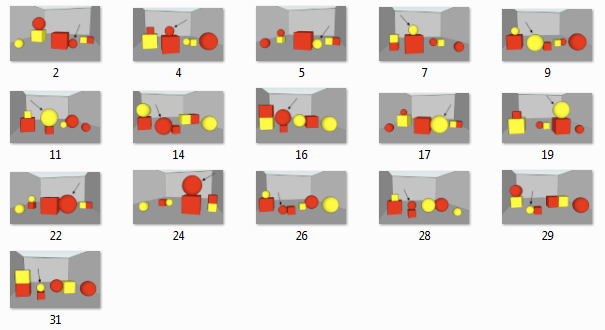
\includegraphics[width=1\textwidth]{images/rojo-amarillo.png}
%\caption{Im\'agenes del \textit{GRE3D7} parte rojo y amarillo}
%\label{rojo-amarillo}
%\end{figure}

\subsection{Calculando \puse\ cuando hay disponible un corpus para la escena considerada}
\label{sec:learning-corpus}

Supongamos que queremos generar autom\'aticamente una ER para el target $t$ en una
determinada escena, y que tenemos disponible un corpus $C$ de ERs de $t$
en esa escena (esto es exactamente el tipo de informaci\'on que encontramos en el
\textit{GRE3D7} corpus \textit{y en el TUNA-corpus}).

En la Figura \ref{verde-azul} se muestran las escenas mostradas a los participantes del corpus \textit{GRE3D7} introducido en la Secci\'on \ref{sec:corpusGRE}, esta parte incluye s\'olo las escenas verde y azules. El corpus contiene otra parte similar con colores rojo y amarillo.

\begin{figure}[H]
\centering
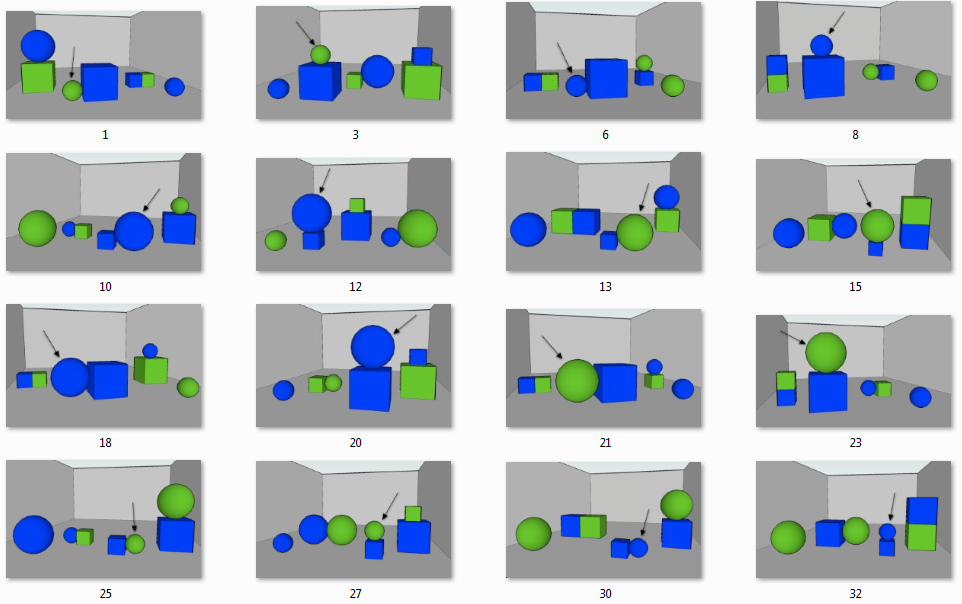
\includegraphics[width=1\textwidth]{images/corpusVerdeAzul.png}
%\vspace{-0.5}
\caption{Im\'agenes del \textit{GRE3D7} parte azul y verde.}
\label{verde-azul}
\end{figure}

El corpus tiene para cada imagen 140 ERs dadas por personas. La Figura \ref{fig4-4} muestra una escena y las distintas ERs que aparecieron en el corpus para esa escena.
\begin{figure}[H]
\begin{minipage}[b]{0.5\linewidth}
\centering
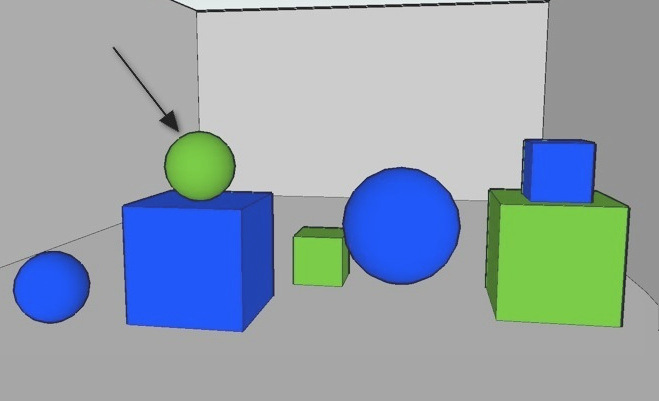
\includegraphics[width=\textwidth]{images/3.jpg}
%\vspace*{1cm}
%\caption{Contexto 3 del GRE3D7}
\end{minipage}
\hspace*{1cm}
\begin{minipage}[b]{0.5\linewidth}
\footnotesize{
{\it green ball} \\
{\it small green ball}  \\
{\it small green ball on top of large red cube} \\
{\it green ball on top of blue cube}\\
{\it green ball on top of large blue cube} \\
{\it small green ball on top of blue cube}  \\
{\it ball on top of cube} \\
{\it small green ball on top of red large left cube}  \\
{\it small ball on top of cube large}  \\
{\it top green ball}   \\
{\it small ball on top of cube } \\
{\it green ball on top of cube }

%green ball \\
%small green ball  \\
%small green ball on-top red large cube \\
%green ball on-top blue cube\\
%green ball on-top large blue cube \\
%small green ball on-top blue cube  \\
%ball on-top cube \\
%small green ball on-top red large left cube  \\
%small ball on-top cube large  \\
%top green ball   \\
%small ball on-top cube  \\
%green ball on-top cube  \\
}
\end{minipage}
\caption{ERs dadas por las personas que completaron el experimento del corpus \textit{GRE3D7} para el contexto de la imagen.}\label{fig4-4}
\end{figure}
Las ERs dadas en Figura \ref{fig4-4} son las ERs diferentes que est\'an en el corpus para el contexto mostrado en la misma figura. Viendo esas ERs, uno podr\'ia imaginarse que no son las del corpus mismo, ya que diferentes personas normalmente usan distintas palabras para nombrar al mismo objeto, distintas frases, distinto orden de las palabras, s\'i es verdad, este corpus ya ha sido procesado para filtrar todas esas cosas, dejar un vocabulario com\'un a todas las ERs, si bien es verdad que con eso perdemos informaci\'on por ejemplo de la realizaci\'on particular que hizo una persona, pero ganamos en poder agrupar las ERs por la informaci\'on que la persona incluy\'o, en la etapa de selecci\'on de contenido de la ER. Si quisieramos partir de un corpus con las ERs tal cual dieron las personas, tendr\'iamos que realizar los siguientes pasos a fin de unificar el vocabulario:

Antes de dar la metodolog\'ia para calcular las probabilidades de uso, explicaremos qu\'e hacer con un corpus de ERs para tener unificado el vocabulario, recordemos que el objetivo de la tesis se centra en la selecci\'on de contenidos de las ERs y por ello, no vamos a prestar atenci\'on a la realizaci\'on particular que di\'o cada persona de la ER. 

\begin{enumerate}
\item \textbf{Tokenizar} las expresiones referenciales y llamar al conjunto de palabras distintas
 $Pal$. En particular, las expresiones de varias palabras como {\it arriba de}, {\it encima de}
  deben ser igualadas a una \'unica palabra que signifique lo mismo, digamos \emph{ontop}.

\item \textbf{Eliminar hiper\'onimos} de $Pal$. Por ejemplo, si ambos \emph{cube} y
  \emph{cosa} aparecen en $Pal$ para nombrar la misma cosa, eliminar \emph{cosa}, ya que \emph{cube} es m\'as espec\'ifico.

\item \textbf{Normalizar sin\'onimos} si el conjunto de palabras obtenidas en los pasos anteriores contiene
  sin\'onimos hay que normalizarlos con un representante de la clase. Por ejemplo, las palabras \emph{chico}
  y \emph{peque\~no} son ambas representadas por la palabra \emph{small}.

\item \textbf{Llamar $\REL$} al conjunto resultante, de la etapa anterior; que ser\'a la signatura del modelo $\gM$ que utilizar\'a el algoritmo.

\item \textbf{Definir $\gM$} para cada escena, tal que la interpretaci\'on
 $\interp {\cdot}$ asegure de que todas las ERs encontradas en el corpus sean ERs en
  el modelo. Por ejemplo, las ERs de \ref{fig4-4} deben denotar el target se\~nalado en la figura, siendo el modelo 
$\gM$ considerado el representado en Figura~\ref{fig4-5}.
%GRE3D7-stimulus-cap2
\item \textbf{Calcular R.\puse\ }para cada R$\in \REL$ utilizando la siguiente f\'ormula: Si
  hay muchas ERs para cada escena (como es el caso del corpus \textit{GRE3D7}) $R.\puse\ = \#ERs$ que tienen R $/\#ERs$ en el corpus
    
  o asignamos 1 a R.\puse \ si R est\'a en la ER, asignamos 0 en caso contrario (como es el caso del corpus TUNA).
\end{enumerate}

En el caso del corpus \textit{GRE3D7} el vocabulario unificado y la signatura del modelo es 
$\REL = \{ball, cube, large, small, green, red, yellow, blue, right, left, top, center, rightof, leftof, ontop,\\ 
bellow\} $

En lo que sigue daremos la definici\'on de regresi\'on lineal que es lo que usaremos para estimar las probabilidades de uso \puse\ de las palabras que le daremos al algoritmo, y luego daremos un ejemplo de c\'omo calculamos las probabilidades de uso para una figura particular del \textit{GRE3D7}.

La \textbf{regresi\'on lineal} es un modelo matem\'atico usado para aproximar la relaci\'on de dependencia entre una variable dependiente Y, las variables independientes $X_i$ y un t\'ermino aleatorio $\varepsilon$. Este modelo puede ser expresado como:

    $Y_t = \beta_0 + \beta_1 X_1 + \beta_2 X_2 + \cdots +\beta_p X_p + \varepsilon$

donde:

    $Y_t$: variable dependiente, explicada o regresando.
    $X_1$, $X_2$, $\cdots$, $X_p$ : variables explicativas, independientes o regresores.
    $\beta_0$,$\beta_1$,$\beta_2$,$\cdots$,$\beta_p$ : par\'ametros, miden la influencia que las variables explicativas tienen sobre Y.

donde $\beta_0$ es la intersecci\'on o t\'ermino {\it constante}, las $\beta_i$ \ (i > 0) son los par\'ametros respectivos a cada variable independiente, y $p$ es el n\'umero de par\'ametros independientes a tener en cuenta en la regresi\'on.

Tomaremos la parte azul y verde del corpus \textit{GRE3D7} mostrado en la Figura \ref{verde-azul}, para aprender las probabilidades de uso de cada palabra de las ERs que dieron las personas, y as\'i darnos una idea de como es la distribuci\'on del uso de las palabras del conjunto $REL$ en el corpus.

Hemos seleccionado algunas propiedades, las cuales las sacamos autom\'aticamente del XML del corpus, nuestro objetivo principal, en esta secci\'on, es conseguir un conjunto de propiedades que son las variables $X_i$ que le daremos al m\'etodo de regresi\'on lineal para calcular la dependencia o independencia de la probabilidad de uso \puse\ de cada palabra con respecto a esas propiedades.

\begin{small}
\begin{table}[H]
\begin{center}
\begin{tabular}{|l|p{10cm}|}
\hline
target-tiene & cuando el elemento target tiene la propiedad. \\
\#rel-prop & n\'umero de propiedades y relaciones que el target tiene.\\
\#rel & n\'umero de relaciones que el target tiene. \\
landmark-tiene & cuando un landmark del target tiene la propiedad, un objeto es un landmark si tiene una relaci\'on directa en el modelo, con el target (lo usamos para el \textit{GRE3D7}).\\
location-has & cuando la RE puede usar la ubicaci\'on del target en la figura (esto se hizo porque el TUNA corpus tiene algunas ER donde se le dijo a la gente que pod\'ian usar la localizaci\'on del objeto).\\
discriminaci\'on (disc) & calculada como 1 sobre el n\'umero de objetos en el modelo que tienen la propiedad.  \\
adj-target-tiene & calculada como la cantidad de adjetivos que la ER contiene.\\
\hline
\end{tabular}
\caption{Caracter\'isticas usadas para conseguir f\'ormulas con regresi\'on lineal que nos den una idea de la probabilidad de uso de cada palabra.} 
\label{features}
\end{center}
\end{table}
\end{small}

El procedimiento entonces fue el siguiente:
Creamos un archivo por cada palabra del vocabulario, es decir por ejemplo para ball, cube, small, red, etc. En cada l\'inea del archivo 
se escribieron la lista de propiedades nombradas anteriormente en la Tabla \ref{features}, para la imagen considerada. Como en total 
fueron consideradas 16 im\'agenes, la primer l\'inea contenia la lista de propiedades calculadas desde el corpus de la Figura 1 del \textit{GRE3D7}, 
la segunda l\'inea del de la Figura 3, y as\'i sucesivamente para todas las figuras que se muestran en la Figura \ref{verde-azul}. 
Cada archivo (uno por cada propiedad o relaci\'on del vocabulario) fue analizado con la funci\'on de regresi\'on lineal del paquete WEKA 
\cite{Hall:WEK09}, que tiene una colecci\'on de herrramientas para aprendizaje autom\'atico.

En la Tabla \ref{tabla-linear-regresion-all} se muestran 4 columnas: en la primer columna podemos ver la palabra, 
en la segunda columna est\'a el error promedio dado por regresi\'on lineal, en la tercera columna el error medio 
y en la cuarta la f\'ormula que regresi\'on lineal calcul\'o para la probabilidad de uso de la palabra considerada.

\begin{table}[H]
\begin{center}
\begin{tabular}{|l|c|c|l|}
\hline
Palabra &Error promedio	LR	& Error-PM	& F\'ormula de LR\\
\hline
ball		 &0.0465   &0.0609	  & 0.2894 * disc + 0.7883\\
\hline
cube		 &0.0417	 &0.0531	  &0.49   * disc - 0.0129\\
\hline
\hline
blue		 &0.0353	 &0.0454	  &0.848  * target-tiene + 0.1073\\
\hline
green		 &0.0264	 &0.046	    &0.8722 * target-tiene + 0.0016\\
\hline
\hline
large		 &0.1762	 &0.2378	  &0.5911 * target-tiene + 0.0354\\
\hline
small		 &0.1499	 &0.1755	  &0.3918 * target-tiene + 0.2478 * landmark-tiene -\\
				 &				 &					&0.0913\\
\hline
\hline
leftof  &0.0041	 &0.0094	  &0.0131 * target-tiene +\\
				 &				 &					&0.0253 * adj-target-tiene - 0.0507\\
\hline
ontop	 &0.0706	 &0.1594	  &0.2942 * target-tiene \\
\hline
rightof &0.0029	 &0.0049	  &0.0153 * target-tiene + 0.001\\
\hline
\hline
left		 &0.0068	 &0.0101	  &0.0346 * adj-target-tiene - 0.0653\\
\hline
right		 &0.0079	 &0.0092	  &-0.0118 * disc + 0.0141\\
\hline
top    &0.0099 	 &0.0135		& 0.0069\\
\hline
center	 &0.0023	 &0.0037	  &0.0047 * target-tiene + 0.0047 * adj-target-tiene +\\
				 &				 &					&0.0029 * landmark-tiene - 0.009\\
\hline
\end{tabular}
\caption{F\'ormulas y errores de regresi\'on lineal para la parte del corpus \textit{GRE3D7} que se muestra en la Figura \ref{verde-azul}.}
\label{tabla-linear-regresion-all}
\end{center}
\end{table}

Las palabras {\it red} y {\it yellow} no aparecen en la Tabla \ref{tabla-linear-regresion-all} porque no aparec\'ian en las ERs del corpus de las im\'agenes consideradas (las que conten\'ian colores verdes y azules).

%\textbf{A ESTA TABLA LE FALTAN 3... DEBERIA AGREGARLAS!}

%En la Tabla \ref{tabla-linear-regresion-all} se muestran 4 columnas: en la primer columna podemos ver la palabra, 
%en la segunda columna est\'a el error promedio dado por regresi\'on lineal, en la tercera columna el error medio 
%y en la cuarta la f\'ormula que regresi\'on lineal calcul\'o para la probabilidad de uso de la palabra considerada. 

Podemos ver por ejemplo que {\it ball} tiene una \puse\ alta, es natural ya que en el corpus todos los targets son {\it ball}, como se v\'e en la Figura \ref{verde-azul}, en cambio se puede ver que {\it cube} no es tan alta y depende de la discernibilidad, este n\'umero en la \puse\ debe leerse como la probabilidad de usar {\it cube} en la descripci\'on del landmark. En los casos de {\it blue} y {\it green} el valor de \puse\ depende de si el target es {\it blue} o {\it green}, entonces si el target es {\it blue}, le d\'a un valor alto a {\it blue} y bajo a {\it green} y viceversa, no depende del valor de discernibilidad en el modelo. En la tabla tambi\'en podemos ver que relaciones como {\it small} y {\it large} tienen un error mucho m\'as alto que el resto de las relaciones, esto se debe a que ellas son propiedades vagas. Este tipo de propiedades no son absolutas y dependen del contexto considerado.
Las relaciones {\it ontop}, {\it leftof} y {\it rightof} dependen fuertemente si el target tiene o no esa relaci\'on y en caso de tenerla igualmente la \puse\ no es muy alta, esto indica que en un porcentaje del 30\% por ejemplo se usa {\it ontop} y en menos del 3\% {\it leftof} o {\it rightof}, esta observaci\'on fue reportada en (Viethen, 2011). Una caracter\'istica interesante que vemos y que no fue mencionada en trabajo previo es que tama\~no es m\'as frecuente usado para sobreespecificaci\'on cuando el target y el landmark tienen el mismo tama\~no 
(es usado en ERs sobreespecificadas el 49\% cuando el target y el landmark comparten el tama\~no, y s\'olo el 25\% cuando no lo comparten).

 Utilizamos las ER de $C$
para definir el modelo relacional utilizado por el algoritmo. Entonces 
estimaremos el valor de \puse\ para cada una de las relaciones en el modelo como el
porcentaje en que aparece la relaci\'on en las ER. Es decir,
\begin{equation} \label{eq1}
R.\puse = \frac {\#\mbox{de ERs en $C$ en el que aparece R}} {\#\mbox{de las ER en $C$}}.
\end{equation}

Por ejemplo {\it ball} del ejemplo de la Figura \ref{fig4-4}, apareci\'o en todas las ERs del corpus es decir 140, entonces {\it ball}\puse\=1 ya que 140/140=1, en cambio {\it green} apareci\'o en 137 ERs, entonces {\it green}\puse=0.98 ya que 137/140=0.98.

Esta estimaci\'on es simplista y, por ejemplo, no 
diferencia las propiedades del target y las propiedades de
los landmarks utilizadas en una ER relacional para completar la descripci\'on
del target. Pero es intuitiva y no requiere parsear las ERs para distinguir entre target y landmark. Como vamos a ver
en el Cap\'itulo~\ref{sec:evaluacion} produce ERs naturales
que coinciden con las encontradas en corpora.

Veamos ahora el siguiente ejemplo, el contexto y las ERs del corpus para la escena se muestran en la Figura \ref{fig4-4}. Se muestra en la Figura \ref{fig4-5}, el modelo que representa 
las propiedades y relaciones de los objetos del contexto considerado.

\begin{figure}[H]
\centering
\begin{tikzpicture}
  [
    n/.style={circle,draw,inner sep=3pt,node distance=2cm},
    aArrow/.style={->, >=stealth, semithick, shorten <= 1pt, shorten >= 1pt},
  ]
 \node[n,label=below:{
    \relsize{-1}$\begin{array}{c}
      \nLeft\\[-2pt]
      \nSmall\\[-2pt] 
      \nBlue\\[-2pt]
      \nBall\end{array}$}] (a) {$e_1$};

 \node[n,label=below:{
    \relsize{-1}$\begin{array}{c}
      \nLeft\\[-2pt]
      \nBig\\[-2pt] 
      \nBlue\\[-2pt]
      \nCube\end{array}$}, right of=a] (b) {$e_2$};

 \node[n,label=above:{
    \relsize{-1}$\begin{array}{c}
      \nTop\\[-2pt]      
			\nLeft\\[-2pt]
      \nSmall\\[-2pt]      
			\nGreen\\[-2pt]
      \nBall\end{array}$}, above of=b] (c) {$e_3$};

 \node[n,label=below:{
    \relsize{-1}$\begin{array}{c}
      \nSmall\\[-2pt] 
      \nGreen\\[-2pt] 
      \nCube\end{array}$}, right of=b] (d) {$e_4$};

 \node[n,label=below:{
    \relsize{-1}$\begin{array}{c}
      \nBig\\[-2pt] 
      \nBlue\\[-2pt] 
      \nBall\end{array}$}, right of=d] (e) {$e_5$};

 \node[n,label=below:{
    \relsize{-1}$\begin{array}{c}
      \nBig\\[-2pt] 
      \nGreen\\[-2pt] 
      \nCube\end{array}$}, right of=e] (f) {$e_6$};

 \node[n,label=above:{
    \relsize{-1}$\begin{array}{c}
      \nTop\\[-2pt]
      \nSmall\\[-2pt]
      \nBlue\\[-2pt]
      \nCube\end{array}$}, above of=f] (g) {$e_7$};

 \draw [aArrow,bend right=90] (b) to node[auto,swap]{\relsize{-1}$\nBelow$} (c);
 \draw [aArrow,bend right=90] (c) to node[auto,swap]{\relsize{-1}$\nOntop$} (b);

 \draw [aArrow,bend right=30] (d) to node[auto,swap]{\relsize{-1}$\nLeftof$} (e);
 \draw [aArrow,bend right=30] (e) to node[auto,swap]{\relsize{-1}$\nRightof$} (d);

 \draw [aArrow,bend right=90] (f) to node[auto,swap]{\relsize{-1}$\nBelow$} (g);
 \draw [aArrow,bend right=90] (g) to node[auto,swap]{\relsize{-1}$\nOntop$} (f);
\draw[dotted] (-0.5,-2.4) rectangle (10,4.7);
 %\draw[dotted] (-.65,-1.2) rectangle (7.1,2.1);

 \end{tikzpicture}
\vspace*{-.4cm}\caption{Representaci\'on de las propiedades y relaciones, como un grafo etiquetado, del contexto de la Figura \ref{fig4-4}.}
\label{fig4-5}
\end{figure}

Las ERs, cantidad de ocurrencias y porcentaje del corpus para de la Figura~\ref{fig4-4} se muestran en la Tabla~\ref{corpus-distribution}, la signatura resultante y su \puse\ asociado figuran en las dos primeras columnas de la Tabla~\ref{probability-of-use}.\\

\begin{table}[h!]
\begin{center}
\begin{tabular}{|l|c|c|}
\hline
Expresiones Referenciales & Cantidad de ocurrencias & Porcentaje \\
\hline

green ball & 91 & 65.00\% \\
small green ball   & 23 & 16.43\% \\
small green ball on-top red large cube & 8 & 5.71\% \\
green ball on-top blue cube & 5 & 3.57\% \\
green ball on-top large blue cube & 5 & 3.57\% \\
small green ball on-top blue cube & 2 & 1.43\% \\
ball on-top cube & 1 & 0.71\% \\
small green ball on-top red large left cube  & 1 & 0.71\% \\
small ball on-top large cube & 1 & 0.71\% \\
top green ball  & 1 & 0.71\% \\
small ball on-top cube & 1 & 0.71\% \\
green ball on-top cube & 1 & 0.71\% \\

\hline
\end{tabular}
\caption{Sem\'antica de las expresiones referenciales producidas por las personas para la Figura~\ref{fig4-4}.}\label{corpus-distribution}
\end{center}
\end{table}

Observe que los valores R.\puse\ obtenidos de esta manera deben ser
interpretados como la probabilidad de utilizar R para describir el target en
modelo de $\gM $, y podr\'{i}amos argumentar que se correlacionan con la
 saliencia de R para el target y su modelo. Por esa raz\'on, por ejemplo, el
valor de \emph{ball}.\puse\ es 1, mientras que el valor de
\emph{cube}.\puse\ es 0.178. \\

Estas probabilidades no ser\'an \'utiles
para describir los diferentes targets en diferentes escenas. Veremos c\'omo se
pueden utilizarlas para obtener valores para los nuevos targets y escenas utilizando un
enfoque de aprendizaje autom\'atico en la siguiente secci\'on. Como mostramos en el Cap\'itulo~\ref{sec:evaluacion} el algoritmo genera ER
con una distribuci\'on que coincide con la encontrada en el corpus e incluso las ERs generadas por el algoritmo que no se encontraron
en el corpus son naturales.



\subsection{Calculando \puse\ para el target para escenas sin corpus } 
\label{subsec:learning}

%If there is no corpora that describes the target we can estimate the
%\puse~from corpora on a different scenes in the same domain.
%
%We use simple features to obtain the function, all the features can be
%extracted automatically from the relational model and are listed in


Si no hay corpus de expresiones referenciales que describen el target, se puede estimar la \puse~a partir de corpus de
diferentes escenas en el mismo dominio.
Usamos caracter\'isticas simples para obtener una funci\'on que nos dar\'a la probabilidad de cada palabra en el nuevo modelo, todas las caracter\'isticas se pueden extraer de forma autom\'atica desde el modelo relacional y se enumeran en la Tabla~\ref{features}.

\begin{itemize}
\item target-tiene 1 cuando el elemento target tiene la propiedad o sino 0. 
\item \#rel-prop n\'umero relaciones unarias y binarias que el target tiene.
\item \#rel  n\'umero de relaciones binarias que el target tiene. 
\item landmark-tiene cuando un landmark del target tiene la propiedad.
%location-has & cuando la RE puede usar la ubicaci\'on del target en la figura (esto se hizo porque el TUNA corpus tiene algunas ER donde se le dijo a la gente que pod\'ian usar la localizaci\'on del objeto).\\
\item disc calculada como 1 sobre el n\'umero de objetos en el modelo que tienen la propiedad.  
\item adj-target-tiene calculada como la cantidad de adjetivos que la ER contiene.
\end{itemize}

En el caso del \textit{GRE3D7} usamos la parte verde-azul, es decir todas las im\'agenes que tienen colores verde y azul, para acotar el problema, asumiendo que la otra parte dar\'ia algo similar. En la Figura \ref{verde-azul} se muestran los contextos considerados.

Para hacer el aprendizaje, separamos 1 contexto al que llamamos testing, y todos los dem\'as de entrenamiento. Por ejemplo para aprender \puse\ del contexto 13, se usaron los contextos: 1, 3, 6, 8, 10, 12, 15, 18, 20, 21, 23, 25, 27, 30 y 32. Y as\'i sucesivamente para los dem\'as contextos.

Nuestro conjunto de caracter\'{i}sticas es intencionadamente simplista con el fin de que sea
independiente de dominio. Como resultado hay algunas relaciones complejas
entre las caracter\'{i}sticas de las escenas que no es capaz de
capturar. La caracter\'{i}stica m\'as importante del dominio \textit{GRE3D7}
que no somos capaces de aprender, y tiene un impacto en nuestro desempe\~no, es que
las propiedades de tama\~no (es decir, small y large) se utilizan mucho
m\'as cuando el target no puede ser identificado s\'olo con las propiedades taxon\'omicas absolutas 
(verde y azul) y (ball y cube). En otras palabras, en el corpus \textit{GRE3D7} se utiliza el tama\~no con m\'as frecuencia (90,2 \%)
cuando la ER resultante no es sobreespecificada y cuando si es sobreespecificada el (34 \%). 
Puede que no sea posible aprender esta caracter\'{i}stica de los
datos del \textit{GRE3D7} ya que incluso con las funciones que dependen de dominio definidos
en~\cite[Cap\'{i}tulo 6] {viet:gene11}, no pod\'{i}a ser aprendido por \'arboles decisi\'on. 
Como resultado podemos ver en la Tabla~\ref{probability-of-use} de la Figura 13, el valor estimado para 
\emph{large} no est\'a cerca de la
valor calculado a partir de corpus. En el caso del TUNA-corpus
  mostramos que no podemos aprender la dependencia de la dimensi\'on-X y
  dimensi\'on-y, es decir, cuando una persona a\~nade dimensi\'on-x es altamente
  probable que incluya la dimensi\'on-y en su expresi\'on referencial.

\begin{figure}[ht]
\begin{minipage}[b]{0.5\linewidth}
\centering
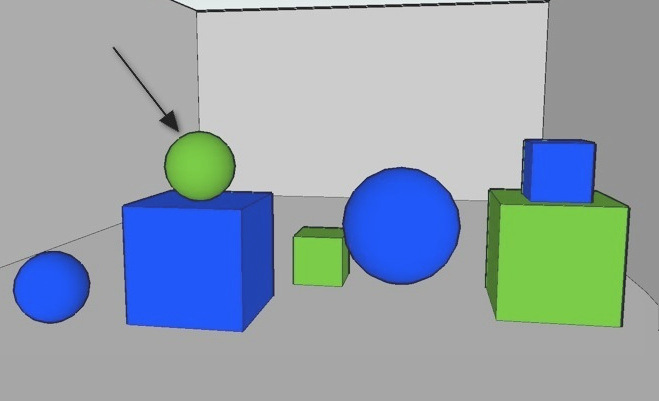
\includegraphics[width=\textwidth]{images/3.jpg}
%\vspace*{1cm}
\caption{Contexto 3 del \textit{GRE3D7}.}
\label{GRE3D7-stimulus-3}
\end{minipage}
%\hspace*{-0.35cm}
\begin{minipage}[b]{0.5\linewidth}
\centering
%\begin{figure}[ht]
%\begin{center}
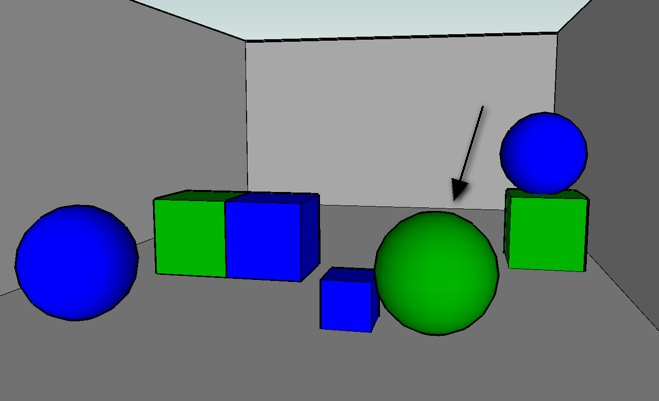
\includegraphics[width=\textwidth]{images/13.jpg}
\caption{Contexto 13 del \textit{GRE3D7}.}
\label{GRE3D7-stimulus-13}
\end{minipage}
\end{figure}

\begin{table}[h!]
\begin{center}
\begin{tabular}{|l|c|c|c|c|}
\hline
%Palabra &  \puse 				 & \puse\ Aprendida 			   & \puse\ & \puse\  Aprendida \\
Palabra & \puse\ Figura \ref{GRE3D7-stimulus-3}   & \puse\ aprendida \ref{GRE3D7-stimulus-3} & \puse\ Figura \ref{GRE3D7-stimulus-13} & \puse\ aprendida \ref{GRE3D7-stimulus-13}  \\
\hline
ball & 1.0 & 1.0 & 1.0 & 1.0 \\
cube & 1.0 & 1.0 & 1.0 & 1.0 \\
green & 0.978 & 0.993 & 1.0 & 0.9875 \\
small & 0.257 & 0.346 & 0.0428 & 0.1993 \\
ontop & 0.178 & 0.179 & 0 & 0\\ 
blue & 0.15 & 0.124 & 0.064 & 0.1353 \\
large & 0.107 & 0.03 & 0.307 & 0.7378 \\
left & 0.007 & 0.002 & 0 & 0.0024 \\
top & 0.007 & 0 & 0 & 0 \\
right & 0 & 0.001 & 0.064 & 0.0005 \\
leftof & 0 & 0 & 0 & 0 \\
rightof & 0 & 0 & 0.064 & 0.1023 \\
belowof & 0 & 0 & 0 & 0 \\
\hline
\end{tabular}
\caption{Probabilidades de uso de las palabras del corpus \textit{GRE3D7} para las Figuras \ref{GRE3D7-stimulus-3} y \ref{GRE3D7-stimulus-13}.} 
\label{probability-of-use}
\end{center}
\end{table}


\begin{table}[h!]
\begin{center}
\begin{tabular}{|l|c|c|}
\hline
%Palabra &  \puse 				 & \puse\ Aprendida 			   & \puse\ & \puse\  Aprendida \\
Palabra & \puse\ Figura \ref{GRE3D7-stimulus-3}   &  \puse\ Figura \ref{GRE3D7-stimulus-13} \\
\hline
ball & 1.0 & 1.0  \\
cube & 1.0 & 1.0  \\
green & 0.978 &  1.0  \\
small & 0.257 & 0.0428  \\
ontop & 0.178  & 0 \\ 
blue & 0.15 & 0.064  \\
large & 0.107  & 0.307  \\
left & 0.007  & 0  \\
top & 0.007  & 0 \\
right & 0  & 0.064  \\
leftof & 0  & 0  \\
rightof & 0  & 0.064  \\
belowof & 0  & 0 \\
\hline
\end{tabular}
\caption{Probabilidades de uso de las palabras del corpus \textit{GRE3D7} para las Figuras \ref{GRE3D7-stimulus-3} y \ref{GRE3D7-stimulus-13}.} 
\label{probability-of-use}
\end{center}
\end{table}


\begin{table}[h!]
\begin{center}
\begin{tabular}{|l|c|c|}
\hline
%Palabra &  \puse 				 & \puse\ Aprendida 			   & \puse\ & \puse\  Aprendida \\
Palabra &  \puse\ aprendida \ref{GRE3D7-stimulus-3} & \puse\ aprendida \ref{GRE3D7-stimulus-13}  \\
\hline
ball &  1.0 & 1.0 \\
cube &  1.0 & 1.0 \\
green &  0.993 & 0.9875 \\
small &  0.346 & 0.1993 \\
ontop &  0.179 & 0\\ 
blue &  0.124  & 0.1353 \\
large &  0.03  & 0.7378 \\
left &  0.002  & 0.0024 \\
top &  0 & 0 \\
right &  0.001 & 0.0005 \\
leftof &  0 &  0 \\
rightof & 0 &  0.1023 \\
belowof & 0 &  0 \\
\hline
\end{tabular}
\caption{Probabilidades de uso aprendidas para las Figuras \ref{GRE3D7-stimulus-3} y \ref{GRE3D7-stimulus-13}.} 
\label{probability-of-use}
\end{center}
\end{table}


El aprendizaje se realiza con el kit de herramientas de aprendizaje autom\'atico
WEKA~\cite{Hall:WEK09}, entrenando con todas las escenas menos una (para la que estamos aprendiendo) se realiz\'o para el corpus \textit{GRE3D7} y el \textit{TUNA-corpus}. Un ejemplo del contenido de los archivos XML del \textit{TUNA-corpus} se muestra en el Ap\'endice \ref{archivos-xml-tuna}. El corpus cuenta con im\'agenes generadas aleatoriamente, por lo tanto las im\'agenes que se muestran en esta tesis, pueden no ser exactamente como las im\'agenes mostradas a los participantes.

Utilizamos regresi\'on lineal para aprender la funci\'on de
\puse\ para cada palabra en la signatura. Para una escena determinada, reemplazamos
las variables de la funci\'on obtenida por los valores de las caracter\'{i}sticas
de la escena que queremos describir.

La regresi\'on lineal nos permite aprender caracter\'{i}sticas interesantes
 del dominio. Para empezar, se aprenden hechos conocidos
como que un determinado {\it color} aparezca en la ER depende en gran medida de si el
target es de ese color, y que no depende de su
poder de discriminaci\'on en el modelo. Por otra parte, vimos que la relaci\'on {\it ontop}
 se utiliza con m\'as frecuencia que las relaciones horizontales
({it right}, {it left}) lo que confirma un hallazgo previo informado
en~\cite{viet:gene11}. Por \'ultimo, vimos en el
\textit{GRE3D7} corpus (que no fue reportado por el trabajo anterior), se utiliza el tama\~no
m\'as frecuentemente de una manera sobreespecificada cuando el
target y el landmark comparten el tama\~no. El {\it tama\~no} fue utilizado en las ER de manera sobreespecificada en el 49 \% de
las descripciones de escenas en las que el target y el landmark compart\'ian el tama\~no,
y el 25 \% cuando target y el landmark no lo compart\'ian. Esto puede explicarse por la observaci\'on de que si el landmark y el target comparten una propiedad, esta propiedad es m\'as relevante.

\section{El algoritmo probabil\'istico}
\label{sec:algoritmo_probabilistico}
Antes de empezar explicando el algoritmo, daremos algunos conceptos de teor\'ia de modelos necesarios para entenderlo.

Una \textbf{f\'ormula} corresponde a una descripci\'on de uno o m\'as elementos del contexto y puede ser o no una ER dependiendo de 
si su interpretaci\'on coincide o no con el target. Por ejemplo la interpretaci\'on de la f\'ormula \texttt{ball} son todas las esferas 
del contexto. En el contexto de la Figura \ref{figura-y-modelo} ser\'ian: $e_1$, $e_3$ y $e_5$  as\'i como $\interp{\texttt{ball} \land \texttt{yellow}}$ es: $e_1$ y $e_3$.
Como dijimos anteriormente la \textbf{interpretaci\'on de una f\'ormula} es el conjunto de elementos que satisfacen la f\'ormula. A la interpretaci\'on de una f\'ormula tambi\'en la llamaremos \textbf{clase}.

Decimos que una f\'ormula $\exists.R. \phi$ es \textbf{informativa} con respecto a otra f\'ormula $\gamma$ cuando la interpretaci\'on de la conjunci\'on de las dos f\'ormulas ($\exists.R. \phi \land \gamma$) contiene menos elementos que la interpretaci\'on de $\gamma$. Por ejemplo si tenemos la f\'ormula \texttt{ball} y 
queremos saber si \texttt{red} es informativa con respecto a \texttt{ball} para el modelo de la Figura vemos que, s\'i lo es, ya que $e_5$ es una \texttt{esfera roja} y existen otras esferas que no son rojas,
 es decir \texttt{red} divide el conjunto de esferas, por lo tanto es informativa. Si un algoritmo permite agregar f\'ormulas no informativas a las expresiones referenciales, entonces podr\'a generar ERs sobreespecificadas.

Una f\'ormula es \textbf{subsumida} si ya tenemos otras f\'ormulas en RE con m\'as informaci\'on que cubren todo el conjunto de objetos que 
la f\'ormula cubr\'ia. Por ejemplo, $\top$ que es la f\'ormula a la cual todos los objetos pertenecen, ser\'a subsumida cuando se agreguen 
las f\'ormulas \texttt{ball} y \texttt{cube} ya que todos los elementos de la Figura \ref{figura-y-modelo} son o esferas o cubos, 
es decir ya tenemos informaci\'on m\'as precisa de los objetos que $\top$. Formalmente $\interp{\top}$ = \{$e_1$,$e_2$,$e_3$,$e_4$,$e_5$,$e_6$, $e_7$\}, y los conjuntos \interp{\texttt{ball}}=\{$e_1$,$e_3$,$e_5$\} y la \interp{\texttt{cube}}=\{$e_2$,$e_4$,$e_6$,$e_7$\}. La uni\'on de los conjuntos $\interp{\texttt{ball}}$ y $\interp{\texttt{cube}}$ dan exactamente $\interp{\top}$.

%\textbf{Redundante} es una f\'ormula para la cual ya hay otra f\'ormula la cual tenga los mismos objetos del modelo. Por ejemplo para el 
%contexto de la Figura \ref{figura-y-modelo}, si ya tenemos la f\'ormula \texttt{red ball}, la f\'ormula \texttt{large red ball} es redundante, ya 
%que no agrega informaci\'on porque el conjunto de objetos esferas rojas ya ten\'ia solamente 1 objeto $e_5$. Intuitivamente es redundante cuando no divide a ninguna clase.

\textbf{Trivial} es una f\'ormula para la cual no hay objetos que la satisfagan en el modelo considerado, por ejemplo en el contexto de la 
Figura \ref{figura-y-modelo}, \texttt{large yellow ball} es trivial ya que no hay esferas amarillas grandes en el contexto considerado.

Vamos a utilizar f\'ormulas de el lenguaje de descripci\'on $\el$ de la l\'ogica~\cite{baader03} para describir clases de refinamiento.
Note, sin embargo, que el lenguaje formal utilizado en particular es independiente del algoritmo principal, y diferentes 
funciones add$_{\mathcal {L}}$(R,$\varphi $, \RE) se pueden utilizar en funci\'on del lenguaje en cuesti\'on.

La interpretaci\'on de la f\'ormula de $\el$  $\psi \sqcap \exists $R.$ \varphi$ es el conjunto de todos los elementos que 
satisfagan~$\psi$ y que est\'an relacionados por relaci\'on R con alg\'un elemento que satisface $\varphi $.
Por ejemplo, la interpretaci\'on de la f\'ormula \texttt{ball}$\sqcap$ $\exists$ \texttt{leftof}.\texttt{cube} es el conjunto de todas las esferas 
que est\'an a la izquierda de alg\'un cubo.

\begin{figure}[!t]
\small
\centering
\begin{algorithm}[H]
\floatname{algorithm}{Algoritmo}

%\floatname{algorithm}{Algoritmo}
\dontprintsemicolon
\caption{Computando clases de $\mathcal{L}$-similaridad}\label{algo:bisim-l}
\SetKwInOut{Input}{Entrada}\SetKwInOut{Output}{Salida}
\Input{\footnotesize Un modelo $\gM$ y una lista Rs $\in (\REL \times [0,1])^*$
 de relaciones con sus valores de \puse\, odenados por \puse}
\Output{\footnotesize Un conjunto de f\'ormulas \RE tal que
$\{\interp{\varphi} \mid \varphi \in \RE\}$ es el conjunto de clases de
$\mathcal{L}$-similaridad de $\gM$}

$\RE \leftarrow \{\top\}$\tcp*[f]{\footnotesize descripci\'on m\'as general $\top$ aplica a todos los elementos del contexto.}

%Bloque con error comentado
\For{\em (R,R.\puse) $\in$ Rs}{
	R.\randomuse = Random(0,1)\tcp*[f]{\footnotesize R.\randomuse es la probabilidad de usar R} \;
        R.\incuse = (1 $-$ R.\puse) / MaxIterations\tcp*[f]{\footnotesize R.\puse\ incrementadas por R.\incuse en cada ciclo}
}

\Repeat{\em $\forall$((R,R.\puse) $\in$ Rs).(R.\puse $\ge$ 1)\tcp*[f]{\footnotesize R.\puse\ incrementadas hasta que alcanzan 1}}{
  \While(\tcp*[f]{\footnotesize mientras alguna clase tenga al menos 2 elementos}){\em $\exists (\varphi \in$ \RE)$.(\#\interp{\varphi}>1)$}{
      \RE' $\leftarrow$ \RE \tcp*[f]{\footnotesize hacer una copia para futura comparaci\'on} \;
      \For{\em (R, R.\puse) $\in$ Rs}{
          \If(\tcp*[f]{\footnotesize R ser\'a usada en la expresi\'on}){\em R.\randomuse $\le$ R.\puse}{
              \lFor{\em $\varphi \in$ \RE}{
                  add$_\mathcal{EL}$(R, $\varphi$, \RE)\tcp*[f]{\footnotesize refine todas las clases usando R}}
                  }\;
              \If(\tcp*[f]{\footnotesize la clasificaci\'on cambi\'o}){\em \RE $\not =$ \RE'}{exit\tcp*[f]{\footnotesize salga del ciclo for para tratar de nuevo con la m\'as alta R.\puse}}
              }
     \If(\tcp*[f]{\footnotesize la clasificaci\'on se ha estabilizado}){\em \RE $=$ \RE'}{exit\tcp*[f]{\footnotesize salga del ciclo while para incrementar R.\puse.}}
  }
%	Bloque con error comentado
  \For{\em (R,R.\puse) $\in$ Rs}{
    R.\puse $\leftarrow$ R.\puse $+$ R.\incuse\tcp*[f]{\footnotesize incrementar R.\puse}
  }
}
\end{algorithm}


\begin{algorithm}[H]
\floatname{algorithm}{Algoritmo}

\dontprintsemicolon
\caption{add$_\el$(R, $\varphi$, $\RE$)} \label{algo:bisim-add-el-over}
\SetKwInOut{Input}{Entrada}\SetKwInOut{Output}{Salida}
\Input{\footnotesize R, $\varphi$, $\RE$}
\Output{\footnotesize $\RE$}

\If(\tcp*[f]{\footnotesize primera iteraci\'on?}){\em FirstLoop?}{
    Informativa $\leftarrow$ TRUE \tcp*[f]{\footnotesize permitir sobreespecificaci\'on}}
\lElse(\tcp*[f]{\footnotesize informativa: tiene menos objetos que la original?}) {Informativa $\leftarrow$ $\interp{\psi \sqcap \exists \mbox{\em R}.\varphi} \neq \interp{\psi}$} 
\For{\em $\psi \in \RE$ con $\#\interp{\psi} > 1$}{
  \If{\em $\psi \sqcap \exists$R.$\varphi$ no est\'a subsumida en $\RE$ \ {\bf and} \tcp*[f]{\footnotesize subsumida: su interpretaci\'on es igual a la uni\'on de las interpretaciones de otras f\'ormulas en \RE?}\\
    \em \ \ \ $\interp{\psi \sqcap \exists \mbox{\em R}.\varphi} \neq \emptyset$ {\bf and} \tcp*[f]{\footnotesize es no-trivial: tiene elementos?}\\
     \ \ \  \emph{Informativa}}{
    Agregar $\psi \sqcap \exists \mbox{R}.\varphi$ a $\RE$ \tcp*[f]{\footnotesize agregar la nueva clase a la clasificaci\'on} \;\\
		
    borrar f\'ormulas subsumidas de $\RE$ \tcp*[f]{\footnotesize borrar clases subsumidas}
  }
}
\end{algorithm}
\vspace*{-.5cm}\caption{Algoritmos de refinamiento con probabilidades y sobreespecificaci\'on para el lenguage \el. El lenguaje formal utilizado es independiente del algoritmo principal, y se pueden utilizar diferentes funciones add$_{\mathcal {L}}$(R,$\varphi $, \RE) en funci\'on del lenguaje considerado.}\label{fig:algo3}

\end{figure}

El conjunto $\RE$ contendr\'a la descripci\'on formal de las clases de refinamiento
y es inicializado por la descripci\'on m\'as general $\top$. Al finalizar contendr\'a las f\'ormulas que representan las ERs de los elementos del modelo.

El Algoritmo \ref{algo:bisim-l} realiza los siguientes pasos. Primero, recorre la lista Rs, para cada R (relaciones de la signatura del dominio $REL$), calcula R.\randomuse, un n\'umero aleatorio en [0,1], y R.incuse que ser\'a (1 - R.puse) / MaxIterations, siendo MaxIterations el n\'umero m\'aximo de iteraciones del ciclo principal que queremos permitir. Si R.\randomuse $\le$ R.\puse\ entonces vamos a utilizar R para refinar el conjunto de
clases. El valor de R.\puse\ se incrementar\'a en $R.\incuse$
en cada ciclo principal, para asegurar que todas las relaciones son, en alg\'un momento,
consideradas por el algoritmo. Esto asegura que una expresi\'on referencial
se encontrar\'a si existe; pero dar\'a mayor probabilidad a las expresiones
que usan las relaciones con m\'as alta R.\puse. Mientras que $\RE$ contiene descripciones (f\'ormulas $\varphi$) que pueden ser refinadas,(es decir, clases
con al menos dos elementos) vamos a llamar a la funci\'on de refinamiento
add$_\mathcal{EL}$(R,$\varphi$,$\RE$) sucesivamente con cada relaci\'on
de Rs. Un cambio en una de las clases, puede desencadenar cambios en
las otras. Por esa raz\'on, si $\RE$ cambia, salimos del ciclo for y volvemos a
empezar con las relaciones de m\'as alta R.\puse. Se refinar\'a cada una de las descripciones
en $\RE$ utilizando la relaci\'on R y las otras descripciones que ya est\'an en
$\RE$, bajo ciertas condiciones que se detallan a continuaci\'on: 
La nueva descripci\'on debe ser
\emph{no redundante} (la nueva clase no se puede obtener como la uni\'on de
clases ya representadas en $\RE$), \emph{no trivial} (la nueva
clase no es vac\'{i}a), es \emph{informativa} (la nueva clase no debe
coincidir con la clase original). Si se cumplen todas estas condiciones,
la nueva descripci\'on se a\~nade a $\RE$, y las descripciones redundantes
posiblemente creadas por la adici\'on de la nueva descripci\'on son
eliminadas.
Con respecto a la informatividad, se permitir\'a 

\section{Ejemplo de ejecuci\'on}
\label{sec:ejemplo_ejecucion}

En esta secci\'on vamos a mostrar un ejemplo de ejecuci\'on para el modelo de la Figura \ref{fig4-9}, considerando la probabilidades de uso mostradas en la Tabla\ref{probabilidades-ejemplo-ejecucion}. Mostraremos la ejecuci\'on del algoritmo sin dar un target espec\'ifico. En este caso el algoritmo obtiene ERs para todos los elementos del modelo. Al finalizar entonces esperamos tener una ER para cada elemento del modelo. Por simplicidad no vamos a nombrar cada vez que tal propiedad pas\'o la probabilidad random del algoritmo, pero s\'i lo nombraremos cuando no la haya pasado. Recordemos que para conseguir no-determinismo, el algoritmo tiene un componente random que hace que si la probabilidad de uso es mayor que el n\'umero random calculado en esa ejecuci\'on. 
En el comienzo $RE$=$\{\top\}$ y $\interp{\top}$ = $\{e_1, e_2, e_3, e_4, e_5, e_6, e_7\}$.\\

\begin{table}[H]
\begin{center}
\footnotesize{
\begin{tabular} {  l c c c c c c c c c c c}
\hline
%\multicolumn{1}{c}{}
%&\multicolumn{1}{c}{Domain}
%&\multicolumn{3}{c}{Descriptions}\\

R				&{\it ball}			& {\it cube}	& {\it red}	  & {\it large} & {\it ontop} & {\it yellow} & {\it small} & {\it rightof} & {\it leftof}& {\it top}& {\it left}   \\
\hline \hline
R.\puse	& 1.0			& 1.0		& 0.978	& 0.257      & 0.178     & 0.15       & 0.107    & 0.007    & 0 & 0 &0\\ \hline
%R.\randomuse & 0.32348895 & 0.5607122 &0.8771196 &0.1256972&0.14249319 &0.039857805 &0.70997673&0.21847993&0.8570516\\
R.\randomuse & 0.3234 & 0.5607 &0.8771 &0.1256 &0.1424 &0.0398 &0.7099 &0.2184 &0.8570 &0.8166 &0.2026\\ \hline
R.\incuse & 0&0&0.0044& 0.1486& 0.1644& 0.17& 0.1786& 0.1986& 0.2 & 0.2 & 0.2\\ \hline

\end{tabular}
}
\end{center}
\vspace*{-.5cm} 
\caption{Distribuci\'on de probabilidad de las propiedades y relaciones de la figura de ejemplo, en la primer fila. Probabilidades random del algoritmo en la segunda fila. Incremento para cada relaci\'on en la tercer fila.}\label{probabilidades-ejemplo-ejecucion}
\vspace*{1cm}
\end{table}

%.large->
%ball->
%centre->
%front->
%left-of->0.14249319
%cube->
%green->
%blue->
%small->
%right-of->0.8166528
%on-top->0.20261234
%above-of->0.33460748
%right>0.40872872
%left->0.3704843
%top->0.796795

\begin{figure}[H]
\begin{subfigure}{0.5\linewidth}
\centering
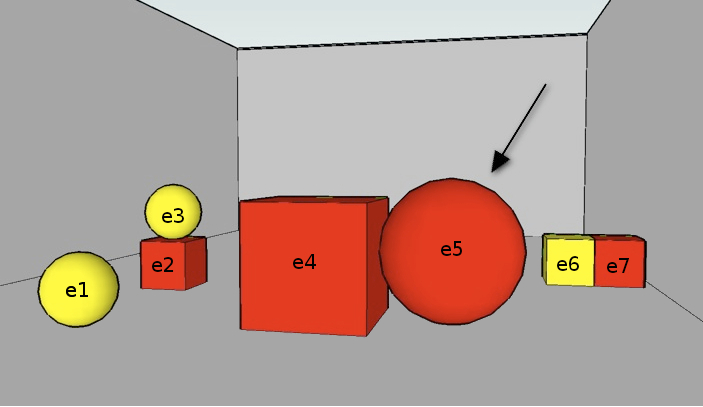
\includegraphics[width=\textwidth]{images/22.jpg}
%\vspace*{1cm}
%\caption{Input scene}
\label{GRE3D7-stimulus-22}
\end{subfigure}
%\hspace*{-0.35cm}
\begin{subfigure}{.5\textwidth}
  \centering
%\includegrahics[width=\textwidth]{images/22sinletras.jpg}
%%\caption{Ejemplo de contexto}
%\label{GRE3D7-stimulus1-b}
%\vspace*{1cm}
\begin{picture}(250,0)
\put(0,-80){\begin{tikzpicture}
  [
    n/.style={circle,draw,inner sep=1.5pt,node distance=1.5cm},
		 aArrow/.style={->, >=stealth, semithick, shorten <= 1pt, shorten >= 1pt},
  ]
 \node[n,label=below:{
    \relsize{-2}$\begin{array}{c}
		  \nLeft\\[-3pt]
      \nSmall\\[-3pt] 
      \nYellow \\[-3pt] 
      \nBall\end{array}$}] (a) {$e_1$};
 \node[n,label=below:{
    \relsize{-2}$\begin{array}{c} 
		  \nLeft\\[-3pt]
      \nSmall\\[-3pt] 
      \nRed\\[-3pt] 
      \nCube\end{array}$}, right of=a] (b) {$e_2$};
 \node[n,label=above:{
    \relsize{-2}$\begin{array}{c}
      \nTop\\[-3pt]
      \nLeft\\[-3pt]
      \nSmall\\[-3pt] 
      \nYellow\\[-3pt] 
      \nBall\end{array}$}, above of=b] (c) {$e_3$};
 \node[n,label=below:{
    \relsize{-2}$\begin{array}{c}
      \nLarge\\[-3pt] 
      \nRed\\[-3pt] 
      \nCube\end{array}$}, right of=b] (d) {$e_4$};
 \node[n,label=below:{
    \relsize{-2}$\begin{array}{c}
      \nLarge\\[-3pt] 
      \nRed\\[-3pt] 
      \nBall\end{array}$}, right of=d] (e) {$e_5$};
 \node[n,label=below:{
    \relsize{-2}$\begin{array}{c}
      \nSmall\\[-3pt] 
      \nYellow\\[-3pt] 
      \nCube\end{array}$}, right of=e] (f) {$e_6$};
 \node[n,label=below:{
    \relsize{-2}$\begin{array}{c}
      \nSmall\\[-3pt]
      \nRed\\[-3pt] 
      \nCube\end{array}$},  right of=f] (g) {$e_7$};
 \draw [aArrow,bend right=40] (b) to node[auto,swap]{\relsize{-3}$\nBelow$} (c);
 \draw [aArrow,bend right=40] (c) to node[auto,swap]{\relsize{-3}$\nOntop$} (b);
 \draw [aArrow,bend right=40] (d) to node[auto,swap]{\relsize{-3}$\nLeftof$} (e);
 \draw [aArrow,bend right=40] (e) to node[auto,swap]{\relsize{-3}$\nRightof$} (d);
 \draw [aArrow,bend right=40] (f) to node[auto,swap]{\relsize{-3}$\nLeftof$} (g);
 \draw [aArrow,bend right=40] (g) to node[auto,swap]{\relsize{-3}$\nRightof$} (f);
 %\draw[dotted] (-0.5,-1.3) rectangle (8,3.1);
 \draw[dotted] (-0.5,-1.8) rectangle (8,3.7);
 \end{tikzpicture}}
 \end{picture}
%\end{flushleft}
\end{subfigure}
\caption{Contexto y modelo del ejemplo de ejecuci\'on.}\label{fig4-9}
\end{figure}

Empezamos, estamos en la primer iteraci\'on del algoritmo. La primer relaci\'on a considerar de acuerdo a las R.\puse\ es \texttt{ball}, pasa la probabilidad del del algoritmo (R.randomuse), recordemos que la relaci\'on \texttt{ball} se a\~nadir\'a a $RE$ si su interpretaci\'on 
tiene al menos un elemento, $\interp{\top \cup \texttt{ball}}$\footnote{Como las relaciones unarias se transformaron en binarias, la f\'ormula que el algoritmo agregar\'a ser\'a $\top \cup \exists\ .\texttt{ball}~\top$. Aqu\'i escribimos $\top \cup \texttt{ball}$ por simplicidad.} no tiene que ser vac\'io, y su interpretaci\'on tiene que ser distinta de $\interp{\top}$. Ambas condiciones se cumplen y $RE$ entonces es \{$\top$, \texttt{ball}\}. Se ven los elementos de la f\'ormula \texttt{ball} en el recuadro de la Figura~\ref{fig-modelo3} que enmarca a $e_1$, $e_3$ y $e_5$.

\begin{figure}[ht]
\begin{center}
\frame{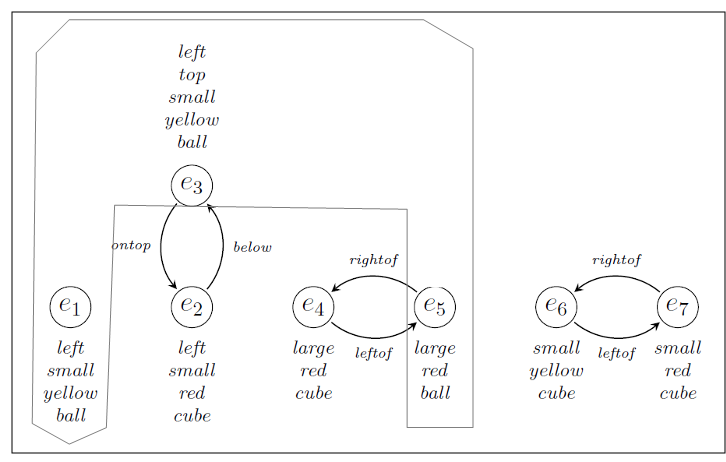
\includegraphics[width=8cm]{images/ej/1ball.png}}\\[0pt]
\caption{El cuadro mayor indica elementos que satisfacen Top. El recuadro m\'as chico elementos que satisfacen la f\'ormula \protect\texttt{ball}.}
\label{fig-modelo3}
\end{center}
\end{figure}

La siguiente propiedad a considerar es \texttt{cube}, tambi\'en pasa la probabilidad del algoritmo (R.randomuse). Realizando el mismo procedimiento antes mencionado, queda $\interp{\texttt{ball}}$ = $\{e_1,e_3,e_5\}$ y
$\interp{\texttt{cube}}$ = $\{e_2, e_4, e_6, e_7\}$. $RE$ =\{$\top$, \texttt{ball}, \texttt{cube}\}. Notar que las particiones de  \texttt{ball} y \texttt{cube} hacen que $\top$ no agregue informaci\'on es decir $\top$ est\'a subsumida, por lo tanto podemos borrarla. Quedando las particiones como se muestran en la Figura~\ref{fig-modelo4}.

%\setlength{\unitlength}{1cm}
%
%\newsavebox{\mybox} 
%\savebox{\mybox}{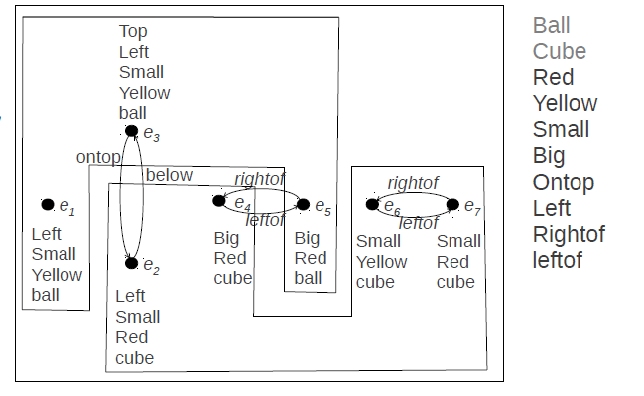
\includegraphics[scale=0.40]{images/modelo4.png}} 
 %\begin{figure}
   %\begin{picture}(8,6)
  %\put(0,0){\usebox{\mybox}} 
  %%\put(2,2.5){\oval(6,5)}
   %\end{picture}   
 %\end{figure} 

\begin{figure}[ht]
\begin{center}
\frame{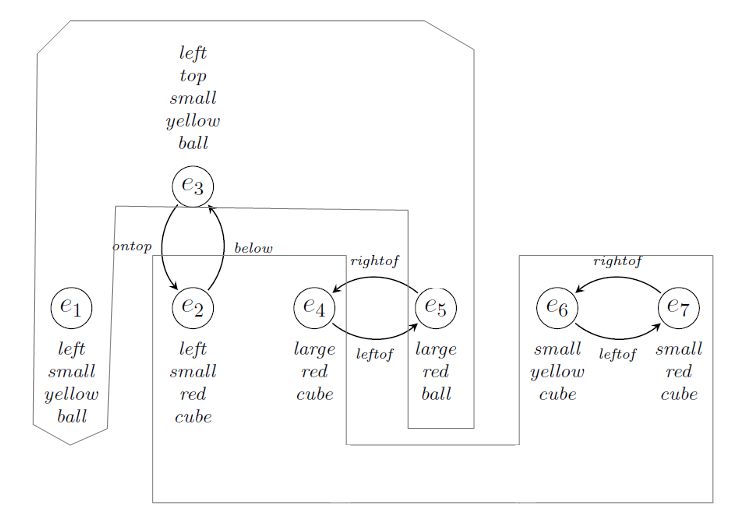
\includegraphics[width=8cm]{images/ej/2ball-cube.png}}\\[0pt]
\caption{Particiones de elementos que satisfacen la f\'ormula \texttt{ball} y otros la f\'ormula \texttt{cube}.}
\label{fig-modelo4}
\end{center}
\end{figure}

La siguiente propiedad es \texttt{red}, pasa la probabilida R.randomuse, tenemos,  
$\interp{\texttt{red}}$ = $\{e_2, e_4, e_5, e_7\}$, haciendo la intersecci\'on con la $\interp{.}$ de cada f\'ormula en $RE$ obtenemos, 
$\{e_5\}$ y $\{e_2, e_4, e_7\}$. Las particiones actuales se pueden ver en la Figura~\ref{fig-modelo9}. El conjunto $RE$ hasta el momento es $\{\texttt{ball}, \texttt{cube}, \texttt{ball} \wedge \texttt{red}, \texttt{cube} \wedge \texttt{red}\}$.

\begin{figure}[ht]
\begin{center}
\frame{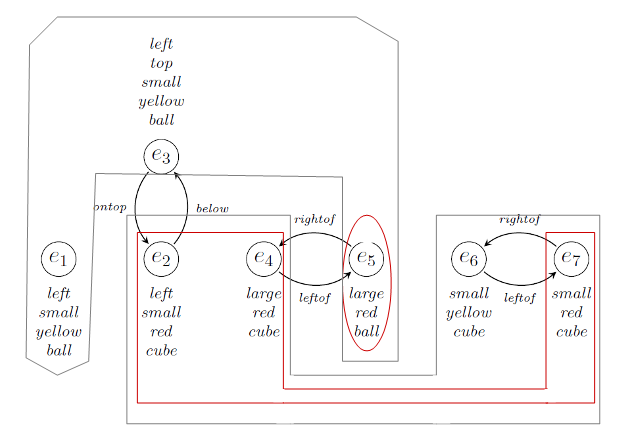
\includegraphics[width=8cm]{images/ej/3ball-cube-red.png}}\\[0pt]
\caption{Cuadros indicando particiones de elementos que cumplen la f\'ormula \texttt{ball}, la f\'ormula \texttt{cube} y la f\'ormula \texttt{red}.}
\label{fig-modelo9}
\end{center}
\end{figure}

Ahora es el turno de \texttt{large} que tambi\'en pasa la probabilidad R.randomuse. Tenemos que $\interp{\texttt{large}}$ = $\{e_4, e_5\}$, haciendo la intersecci\'on con las dem\'as f\'ormulas que tenemos hasta el momento nos queda $RE$ de la siguiente manera:
 $\{\texttt{ball}, \texttt{cube}, \texttt{ball} \wedge \texttt{red} \wedge \texttt{large}, \texttt{cube} \wedge \texttt{red} ,\texttt{cube} \wedge \texttt{red} \wedge \texttt{large} \}$. Notar que en este caso se agreg\'o a a las f\'ormulas $\texttt{ball} \wedge \texttt{red}$ y $\texttt{cube} \wedge \texttt{red}$ porque estamos en la primera iteraci\'on, y no chequeamos informatividad. Las particiones siguen quedando iguales, este es un caso en el que se agrega por sobreespecificaci\'on.
 
La siguiente es \texttt{ontop}, la cual pasa la probabilidad R.randomuse. $e_3$ es el \'unico elemento que esta \texttt{ontop} quedando $RE$= $\{\texttt{ball}, \texttt{cube}, \texttt{ball} \wedge \texttt{red} \wedge \texttt{large}, \texttt{cube} \wedge \texttt{red}, \texttt{cube} \wedge \texttt{red} \wedge \texttt{large}, \texttt{ball} \wedge \exists \Ontop.\texttt{cube} \}$. Las particiones resultantes se muestran en la Figura \ref{new}.


Siguiendo con \texttt{yellow}, tenemos que $\interp{\texttt{yellow}}$ = $\{e_1, e_3, e_6\}$ y obtenemos $RE$= $\{\texttt{ball},\texttt{ball} \wedge \texttt{yellow}, \texttt{cube}, \texttt{cube} \wedge \texttt{yellow}, \texttt{ball} \wedge \texttt{red} \wedge \texttt{large}, \texttt{cube} \wedge \texttt{red}, \texttt{cube} \wedge \texttt{red} \wedge \texttt{large}, \texttt{yellow} \wedge \texttt{ball} \wedge \exists \Ontop.\texttt{cube} \}$. Note que algunas se agregaron sobreespecificando, ya que todav\'ia estamos en el primer ciclo.
Note que aqu\'i ya borramos la f\'ormula \texttt{ball} porque estaba subsumida, y la f\'ormula \texttt{cube} tambi\'en. Se muestran las particiones resultantes en la Figura~\ref{fig-modelo10}.

Las dem\'as propiedades no pasan la probabilidad R.randomuse, por lo tanto salimos del primer ciclo, e incrementamos las probabilidades con R.incuse, quedando como se muestran en la Tabla \ref{prob-inc1}

%Las dem\'as propiedades y no pasaron la probabilidad random del algoritmo, pero a\'un tenemos particiones con m\'as de un elemento, y las probabilidades de uso son menores que 1, por lo tanto se aumentan las probabilidades de uso en 0.2 (siendo ) para cada propiedad quedando:


\begin{table}[H]
\begin{center}
\footnotesize{
\begin{tabular} {  l c c c c c c c c c c c }
\hline
%\multicolumn{1}{c}{}
%&\multicolumn{1}{c}{Domain}
%&\multicolumn{3}{c}{Descriptions}\\

R				&{\it ball}			& {\it cube}	& {\it red}	  & {\it large} & {\it ontop} & {\it yellow} & {\it small} & {\it rightof} & {\it leftof}   & {\it top}& {\it left}   \\
\hline
R.\puse	& 1.0			& 1.0		& 0.9824	& 0.4056 & 0.3424 & 0.32   & 0.2856 & 0.2056& 0.2 &0.2 &0.2  \\
\hline

\end{tabular}
}
\end{center}
\vspace*{-.5cm} 
\caption{Probabilidad de las propiedades y relaciones de la figura de ejemplo, incrementadas en R.\incuse.}\label{prob-inc1}
\vspace*{1cm}
\end{table}

Las interpretaciones hasta el momento son:
$\interp \texttt{ball} = e_1, e_3, e_5 
\interp \texttt{ball} \wedge \texttt{yellow} = e_1, e_3
\interp \texttt{cube} = e_2, e_4, e_6, e_7
\interp \texttt{cube} \wedge \texttt{yellow} = e_6
\interp \texttt{ball} \wedge \texttt{red} \wedge \texttt{large} = e_5
\interp \texttt{cube} \wedge \texttt{red} = e_2, e_4, e_7
\interp \texttt{cube} \wedge \texttt{red} \wedge \texttt{large} = e_4 
\interp \texttt{yellow} \wedge \texttt{ball} \wedge \exists \Ontop.\texttt{cube} = e_3 $

\texttt{ball} y \texttt{cube} est\'an subsumidas, se puede eliminar

$\interp \texttt{ball} \wedge \texttt{yellow} = e_1, e_3
\interp \texttt{cube} \wedge \texttt{yellow} = e_6
\interp \texttt{ball} \wedge \texttt{red} \wedge \texttt{large} = e_5
\interp \texttt{cube} \wedge \texttt{red} = e_2, e_4, e_7
\interp \texttt{cube} \wedge \texttt{red} \wedge \texttt{large} = e_4 
\interp \texttt{yellow} \wedge \texttt{ball} \wedge \exists \Ontop.\texttt{cube} = e_3 $

De ahora hasta que termine, no se agregar\'an propiedades por sobreespecificaci\'on, notar que tenemos 4 conjuntos singleton, los cuales no cambiaran hasta el final de la ejecuci\'on. El algoritmo contin\'ua porque siguen quedando clases para refinar, las cuales son \texttt{ball} \wedge \texttt{yellow} y \texttt{cube} \wedge \texttt{red}.


%Otra vez las probabilidades random superan a las de la lista, recalculamos las probabilidades sumando R.\incuse a cada \puse, quedando como muestra la Tabla \ref{probabilidades-ejemplo-ejecucion3}.

%\begin{table}[H]
%\begin{center}
%\footnotesize{
%\begin{tabular} {  l c c c c c c c c c }
%\hline
%%\multicolumn{1}{c}{}
%%&\multicolumn{1}{c}{Domain}
%%&\multicolumn{3}{c}{Descriptions}\\

%R				&{\it ball}			& {\it cube}	& {\it red}	  & {\it large} & {\it ontop} & {\it yellow} & {\it small} & {\it rightof} & {\it leftof}   \\
%\hline
%R.\puse	& 1.0			& 1.0		& 0.9868	& 0.5542 & 0.5068 & 0.49   & 0.4642 & 0.4042& 0.4 \\
%\hline

%\end{tabular}
%}
%\end{center}
%\vspace*{-.5cm} 
%\caption{Probabilidad de las propiedades y relaciones de la figura de ejemplo, incrementadas en R.\incuse.}\label{probabilidades-ejemplo-ejecucion3}
%\vspace*{1cm}
%\end{table}


\begin{figure}[ht]
\begin{center}
\frame{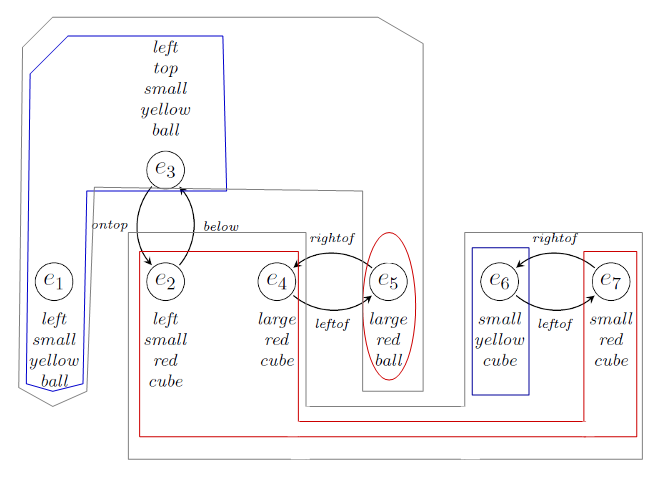
\includegraphics[width=8cm]{images/ej/4ball-cube-red-yellow.png}}\\[0pt]
\caption{Cuadros indicando particiones de elementos que cumplen las f\'ormulas \texttt{ball}, \texttt{cube}, \texttt{red} y \texttt{yellow}.}
\label{fig-modelo10}
\end{center}
\end{figure}

Borrando subsumidas del modelo tenemos
\begin{figure}[ht]
\begin{center}
\frame{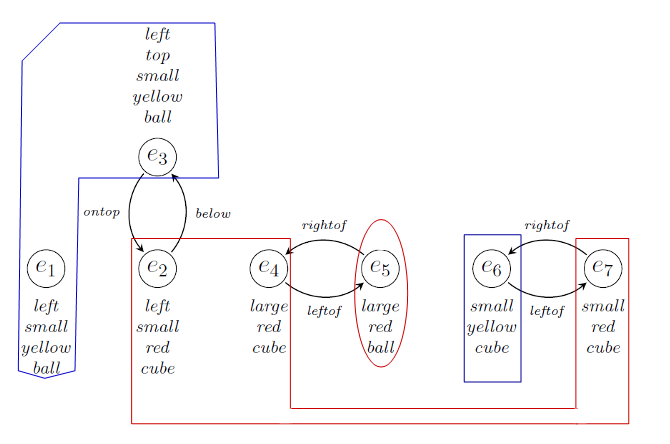
\includegraphics[width=8cm]{images/ej/4b.png}}\\[0pt]
\caption{Cuadros indicando particiones de elementos que cumplen las f\'ormulas \texttt{ball}, \texttt{cube}, \texttt{red} y \texttt{yellow}, sin subsumidas.}
\label{fig-modelo10}
\end{center}
\end{figure}

Haciendo lo mismo con \texttt{small} tenemos $RE$ = $\{\texttt{ball} \wedge \texttt{yellow} \wedge \texttt{small}, \texttt{cube} \wedge \texttt{yellow} \wedge \texttt{small}, \texttt{ball} \wedge \texttt{red}, \texttt{cube} \wedge \texttt{red}, \texttt{cube} \wedge \texttt{red} \wedge \texttt{small}\}$, las particiones resultantes se pueden ver en Figura~\ref{fig-modelo11}.

%\setlength{\unitlength}{1cm}
%
%\newsavebox{\mybox} 
%\savebox{\mybox}{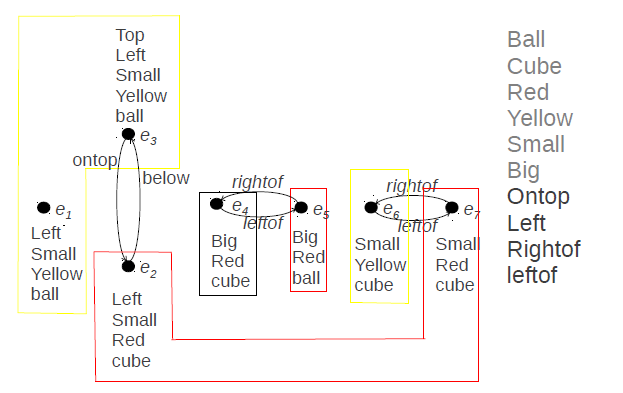
\includegraphics[scale=0.40]{images/modelo11.png}} 
 %\begin{figure}
   %\begin{picture}(8,6)
  %\put(0,0){\usebox{\mybox}} 
  %%\put(2,2.5){\oval(6,5)}
   %\end{picture}   
 %\end{figure} 

\begin{figure}[ht]
\begin{center}
\frame{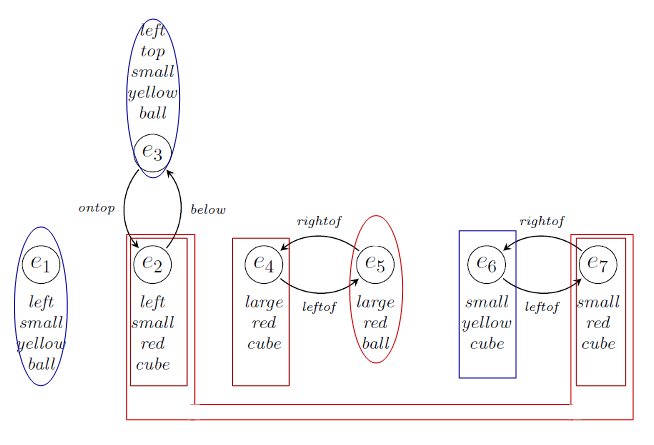
\includegraphics[width=8cm]{images/ej/5ball-cube-red-yellow-large-small.png}}\\[0pt]
\caption{Cuadros indicando \texttt{ball}, \texttt{cube}, \texttt{red}, \texttt{yellow}, \texttt{small} y \texttt{large}.}
\label{fig-modelo11}
\end{center}
\end{figure}

La siguiente propiedad es \texttt{large} as\'i, tenemos $RE$ = $\{\texttt{ball} \wedge \texttt{yellow} \wedge \texttt{small}, \texttt{cube} \wedge \texttt{yellow} \wedge \texttt{small}, \texttt{ball} \wedge \texttt{red}, \texttt{cube} \wedge \texttt{red} \wedge \texttt{large}, \texttt{cube} \wedge \texttt{red} \wedge \texttt{small}\}$. Aqu\'i no podemos agregar \texttt{large} a la f\'ormula $\texttt{red} \wedge \texttt{cube}$ porque su interpretaci\'on tiene un s\'olo elemento, y la condici\'on dice que es necesario tener m\'as de uno (y no estamos en el primer ciclo).

Hasta ahora $RE$ = $\{\texttt{ball} \wedge \texttt{yellow} \wedge \texttt{small}, \texttt{cube} \wedge \texttt{yellow} \wedge \texttt{small}, \texttt{ball} \wedge \texttt{red}, \texttt{cube} \wedge \texttt{red} \wedge \texttt{large}, \texttt{cube} \wedge \texttt{red} \wedge \texttt{small}\}$ 
y tenemos las siguientes extensiones: $\{e_1, e_3\}, \{e_6\}, \{e_5\}, \{e_4\}, \{e_2, e_7\}$ respectivamente. 
Hay dos f\'ormulas que a\'un pueden ser refinadas, $\texttt{ball} \wedge \texttt{yellow} \wedge \texttt{small}$ y $\texttt{cube} \wedge \texttt{red} \wedge \texttt{small}$ 
debido a que tienen m\'as de un elemento cada una, por lo que entran en el ciclo, while del Algoritmo \ref{algo:bisim-l}. Ahora es el turno de las relaciones, la primera de ellas es \texttt{leftof}, para cada f\'ormula $\varphi$ en $RE$ trataremos de hacer add$_\el$ (\texttt{leftof},$\varphi$, $RE$). Notar que $\psi$ solo puede ser $\texttt{ball} \wedge \texttt{yellow} \wedge \texttt{small}$ o $\texttt{cube} \wedge \texttt{red} \wedge \texttt{small}$ porque estas tienen en su interpretaci\'on m\'as de un elemento. 


\begin{figure}[ht]
\begin{center}
\frame{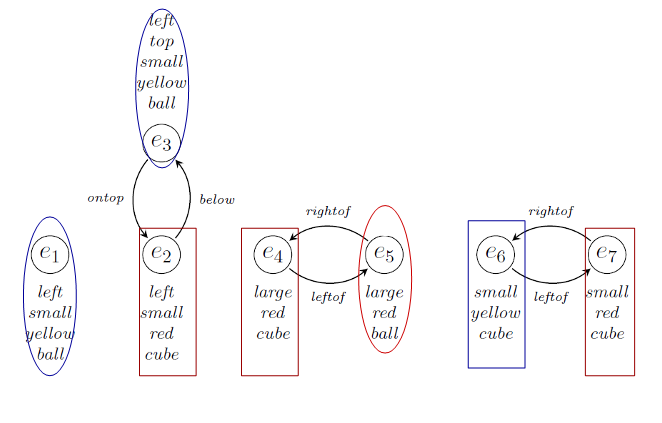
\includegraphics[width=8cm]{images/ej/5b.png}}\\[0pt]
\caption{Cuadros indicando ``ball'', ``cube'', ``red'', ``yellow''...}
\label{fig-modelo15}
\end{center}
\end{figure}


No hay
%because those are the ones that its interpretation have more than one element. There is not 
$\varphi$ y $\psi$ que puedan ser aplicadas. Continuando con \texttt{rightof} agregamos $\texttt{cube} \wedge \texttt{yellow} \wedge \texttt{small} \wedge \exists \texttt{rightof}. \texttt{cube} \wedge \texttt{red} \wedge \texttt{small}$, y as\'i con \texttt{ontop} agregamos $\texttt{small} \wedge \texttt{red} \wedge \texttt{cube} \wedge \exists \texttt{ontop}. \texttt{small} \wedge \texttt{yellow} \wedge \texttt{ball}$ y el algoritmo termina con ER = $\{\texttt{ball} \wedge \texttt{yellow} \wedge \texttt{small}, \texttt{cube} \wedge \texttt{yellow} \wedge \texttt{small}, \texttt{ball} \wedge \texttt{red}, \texttt{cube} \wedge \texttt{red} \wedge \texttt{large}, \texttt{cube} \wedge \texttt{red} \wedge \texttt{small}, \texttt{cube} \wedge \texttt{yellow} \wedge \texttt{small} \wedge \exists \texttt{rightof}. \texttt{cube} \wedge \texttt{red} \wedge \texttt{small}, \texttt{small} \wedge \texttt{red} \wedge \texttt{cube} \wedge \exists \texttt{ontop}. \texttt{small} \wedge \texttt{yellow} \wedge \texttt{ball}\}$, 
aqu\'i todos los elementos est\'an en una clase singleton y no se puede hacer ning\'un refinamiento m\'as. 
%can be applied to $cubo \wedge red \wedge peque\~no$ but there is no formula which interpretation has more than one element to be apply with this one. The same happen for the other relations, so the algorithm ends.
%its interpretation is $\{e_7\}$ with $\psi$ is $cubo \wedge yellow \wedge peque\~no$, the others combinations can't be apply because they don't do true the preconditions. The following relation is rightof, 

%leftof, rightof, ontopof, bellowof

%At this point we already have the target in a singleton set. So the formula for it is ``red and esfera'', and also for s6 which formula is ``yellow cubo''.\\
%As we show this algorithm depends of the order of properties and relations.\\



\begin{figure}[ht]
\begin{center}
\frame{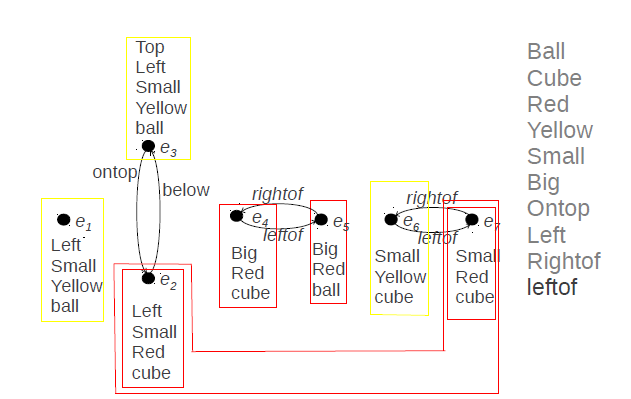
\includegraphics[width=8cm]{images/modelo16.png}}\\[0pt]
\caption{Cuadros indicando ``ball'', ``cube'', ``red'', ``yellow''...}
\label{fig-modelo16}
\end{center}
\end{figure}

\begin{figure}[ht]
\begin{center}
\frame{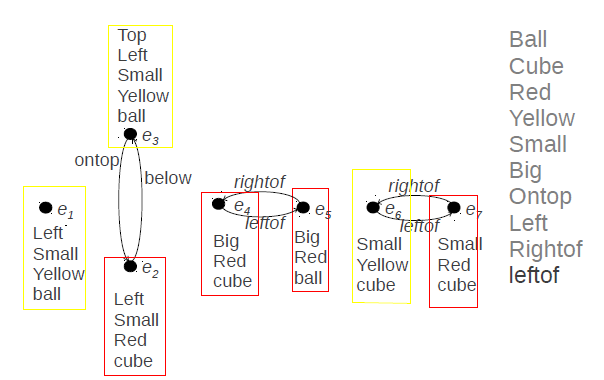
\includegraphics[width=8cm]{images/modelo17.png}}\\[0pt]
\caption{Cuadros indicando ``ball'', ``cube'', ``red'', ``yellow''...}
\label{fig-modelo17}
\end{center}
\end{figure}

Las expresiones referenciales de salida dadas por el algoritmo son:
\begin{itemize}
\item $\texttt{ball} \wedge \texttt{yellow} \wedge \texttt{small}$ representa $e_1$, la cual se puede realizar como \textit{La esfera amarilla peque\~na} 
\item $\texttt{small} \wedge \texttt{red} \wedge \texttt{cube} \wedge \exists \texttt{ontop}. \texttt{small} \wedge \texttt{yellow} \wedge \texttt{ball}$ representa $e_2$, la cual se puede realizar como \textit{El cubo peque\~no y rojo que est\'a arriba de la peque\~na bola amarilla}.
\item $\texttt{cube} \wedge \texttt{red} \wedge \texttt{large}$ representa $e_4$, la cual se puede realizar como \textit{El cubo rojo y grande} 
\item $\texttt{ball} \wedge \texttt{red}$ representa $e_5$, la cual se puede realizar como \textit{La esfera roja} 
\item $\texttt{cube} \wedge \texttt{yellow} \wedge \texttt{small}$ representa $e_6$, que puede realizarse como \textit{El peque\~no cubo amarillo} 
\item $\texttt{cube} \wedge \texttt{red} \wedge \texttt{small}$ representa $\{e_2,e_7\}$, la cual se puede realizar como \textit{Los cubos rojos peque\~nos}  
\item $\texttt{cube} \wedge \texttt{yellow} \wedge \texttt{small} \wedge \exists \texttt{rightof}. \texttt{cube} \wedge \texttt{red} \wedge \texttt{small}$ representa $e_6$, la cual se puede realizar como \textit{El peque\~no cubo amarillo que est\'a a la derecha del peque\~no cubo rojo} 
 
\end{itemize}


\subsection{Asegurando terminaci\'on}

Uno de los problemas que ten\'ian otros algoritmos es que no siempre terminaban, para asegurar terminaci\'on nosotros incrementamos las probabilidades aleatorias en cada ciclo, hasta que alcancen 1. Definimos MaxIterations como la cantidad m\'axima de iteraciones que vamos a permitir, y calculamos R.incuse es cuanto vamos a incrementar la probabilidad de R en cada ciclo, R.incuse = (1 -R.puse) / MaxIterations, con esto nos aseguramos que en MaxIterations todas lleguen a 1, y en consecuencia el algoritmo termine, ya que en el c\'odigo, se incrementa R.puse con R.incuse y sale del ciclo principal si para todas las R, R.puse son mayores o iguales a 1.
Este es un algoritmo de punto fijo, se refinan las particiones hasta que en alg\'un momento no se pueden hacer m\'as refinamientos, se dice que el algoritmo llego a un punto fijo, en el que no le es posible progresar $RE$ se mantiene sin modificaciones. Las particiones se van haciendo m\'as chicas en las sucesivas iteraciones y considerando que la cantidad de elementos del modelo y las relaciones son finitas, el algoritmo siempre termina.

\subsection{Generando ER relacionales}

Nuestro algoritmo permite generar relaciones con otros objetos e incluir expresiones de los dem\'as objetos (no necesariamente ERs), no tiene preferencia por las relaciones ni por las propiedades proposicionales (como otros algoritmos descriptos de trabajo previo), en el sentido de que va o no incluirlas de acuerdo a la probabilidad de uso que ellas tengan, las cuales fueron calculadas o aprendidas de un corpus.

\subsection{Generando ER no-determin\'isticamente}

Al iniciar el algoritmo calcula para cada R, R.\randomuse que es un n\'umero aleatorio entre 0 y 1, ese n\'umero va a hacer que el algoritmo sea no-determin\'istico, ya que, el algoritmo usar\'a R para refinar las clases solamente si 
R.rnduse >= R.puse. Por lo tanto y considerando que en las siguientes ejecuciones R.rnduse ser\'an distintos, va a poder generar distintas ER.

\subsection{Generando descripciones sobreespecificadas}\label{sec:overspecification}

El algoritmo hace caso omiso de la restricci\'on de informatividad (es decir, que permite la inclusi\'on de nuevas relaciones
en la descripci\'on, incluso si no refinan la clase asociada) \emph{pero s\'olo durante el
primer ciclo del algoritmo}. Es decir, durante el primer ciclo sobre los elementos de la
lista de probabilidades Rs, se permitir\'a la inclusi\'on de todas las relaciones que no trivializan la
descripci\'on (es decir, la clase asociada no est\'a vac\'{i}a). Debido a que esto se hace s\'olo durante
el primer ciclo, sabemos que no aparecer\'an propiedades repetidas en las ERs generadas (como \texttt{green green ball}).
En los ciclos restantes, se a\~nadir\'an propiedades adicionales s\'olo si son de car\'acter informativo.
Este dise\~no del algoritmo que permite sobreespecificaci\'on est\'a inspirado en la obra de \cite{keysar:Curr98} sobre el egocentrismo y la producci\'on del lenguaje natural. Keysar et al. argumentan que cuando se produce el lenguaje, el hablante no identifica un\'ivocamente al target desde el principio, sino que  
es m\'as bien un ajuste de \'ultimo momento. Los hablantes producen ERs primero egoc\'entricamente, agregando aquellas propiedades m\'as prominentes por m\'as de que no sean informativas. Pero luego las ajustan de modo que el destinatario de la ER sea capaz de identificarla. El primer paso, egoc\'entrico, es un proceso
heur\'istico basado en un modelo de la prominencia de la propiedades de la escena que contiene el target. Nuestra definici\'on de
\puse\ est\'a destinada a capturar las prominencias de las propiedades de diferentes escenas y targets. Los valores de \puse\
cambian en relaci\'on a la escena considerada. Esto est\'a en contraste con el trabajo previo donde
la prominencia de una propiedad es constante en un dominio. Keysar et al. argumentan que la raz\'on del procedimiento de 
generar-y-ajustar puede tener que ver con las limitaciones de procesamiento de informaci\'on de la
mente: si la heur\'istica que gu\'ia la fase egoc\'entrica est\'a bien sintonizada, consigue una adecuada ER al principio
y rara vez requerir\'a ajustes. Se observa un comportamiento similar
con nuestro algoritmo: cuando los valores de \puse\ son
aprendidos del dominio, el algoritmo no es
s\'olo es m\'as preciso, sino que tambi\'en es mucho m\'as r\'apido que cuando se utilizan valores de \puse\ aleatorios. Por ejemplo la ER \texttt{large red ball} generada por el algoritmo para el target $e_5$ de la Figura \ref{}, las primeras palabras dichas son \texttt{large red} que son las propiedades m\'as sobresaliente del objeto target. 


%\subsection{Generando ER para plurales}
%
%Este algoritmo devuelve ER para todos los elementos del contexto, 
%esto implica que podr\'iamos dar expressiones referenciales de un conjunto de elementos.
%
%Por ejemplo queremos identificar a $e_1$ y $e_5$ 
%siendo resultados dados por el algoritmo que $e_1$
%ball, yellow, small
%y $e_5$ ball, red
%

\section{Notas finales y linkeo del cap\'itulo}
\label{sec:link-algoritmo}

En este cap\'itulo se explic\'o la entrada y salida de un algoritmo probabil\'istico. Una de las entradas es el modelo, el cual es una representaci\'on de la figura considerada. Otra es una distribuci\'on de probabilidades finita, la cual explicamos como obtenerla en 2 casos. Primero en el caso que hay corpus disponible para la escena considerada y en casos donde al no haber corpus disponible proponemos una aproximaci\'on usando aprendizaje autom\'atico. Se explic\'o el algoritmo en detalle y se ilustr\'o con un ejemplo de ejecuci\'on. Se explic\'o c\'omo hace el algoritmo para conseguir las siguientes caracter\'isticas: asegurar terminaci\'on, generar ER relacionales, generar ER no-determin\'isticas y generar sobreespecificaci\'on.
El dise\~no del algoritmo est\'a inspirado en el modelo cognitivo de generaci\'on de expresiones referenciales de \cite{keysar:Curr98}. En el Cap\'itulo \ref{sec:evaluacion} veremos que este algoritmo es capaz de generar rankings de ERs cercanos a los encontrados en corpora.
El algoritmo presentado en este cap\'itulo introduce una familia de algoritmos que extiende probabil\'isticamente a los algoritmos presentados en el Cap\'itulo \ref{sec:intro_logica}. Se explicaron los detalles de la subrutina \textit{add} para el lenguaje \EL. Las definiciones de \textit{add} para otros lenguajes como \ALC o \EPFOL son similares.
Como se discuti\'o en el Cap\'itulo \ref{sec:intro}, los dominios realistas de posibles aplicaciones de la GER contienen incertidumbre. En este cap\'itulo modelamos esa incertidumbre como las probabilidades de usar una caracter\'istica en una ER. 
Estos algoritmos pueden tambi\'en ser usados con probabilidades provenientes de confidence scores de sensores, por ejemplo, para modelar otros tipos de incertidumbre.
En el Cap\'itulo \ref{sec:evaluacion} evaluamos estos algoritmos sobre un corpus de descripciones de mapas, el corpus ZOOM.
% generar ER para plurales.
%
%En el c\'alculo de probabilidades de uso de las palabras con nuestra versi\'on simplista, podemos ver cosas interesantes como por ejemplo que {\it ball} tiene una \puse\ alta, ya que en el corpus considerado todos los targets son {\it ball}, en cambio la probabilidad de {\it cube} no es tan alta y depende de la discernibilidad, si aparece, aparece en la descripci\'on del landmark. Para {\it blue} y {\it green} el valor de \puse\ depende de si el target es {\it blue} o {\it green}, entonces si el target es {\it blue}, le d\'a un valor alto a {\it blue} y bajo a {\it green} y viceversa. Las relaciones {\it ontop}, {\it leftof} y {\it rightof} dependen fuertemente si el target tiene o no esa relaci\'on y en caso de tenerla igualmente la \puse\ no es muy alta, esto indica que en un porcentaje del 30\% por ejemplo se usa {\it ontop} y en menos del 3\% {\it leftof} o {\it rightof}, ya reportado en trabajo previo. Vimos que el tama\~no es m\'as frecuente usado para sobreespecificaci\'on cuando el target y el landmark tienen el mismo tama\~no (es usado en ERs sobreespecificadas el 49\% cuando el target y el landmark comparten el tama\~no, y s\'olo el 25\% cuando no lo comparten).
%Hay algunas relaciones complejas entre las caracter\'{i}sticas de las escenas que no somos capaces de
%capturar. La caracter\'{i}stica m\'as importante del dominio \textit{GRE3D7}
%que no somos capaces de aprender, y tiene un impacto en nuestro desempe\~no, es que
%las propiedades de tama\~no (es decir, small y large) se utilizan mucho
%m\'as cuando el target no puede ser identificado s\'olo con las propiedades taxon\'omicas absolutas 
%(verde y azul) y (ball y cube). En otras palabras, en el corpus \textit{GRE3D7} se utiliza el tama\~no con m\'as frecuencia (90,2 \%)
%cuando la ER resultante no es sobreespecificada y cuando si es sobreespecificada el (34 \%). \\

